% !TEX encoding = UTF-8 Unicode
\documentclass[final]{article}
\usepackage{geoA4}
\usepackage[font=scriptsize]{caption}
\usepackage{libertine}
\usepackage{els}
\usepackage{ii}
\usepackage{notate}
\usepackage{wrapfig}
\newcommand{\ap}{\ensuremath{\tau}\xspace}
\newcommand{\dap}{\ensuremath{d\ap}\xspace}
%\usepackage{geoA4}
\renewcommand{\oe}{;~o.e.{}}
\renewcommand{\ls}{\emph}
\renewcommand{\me}{;~m.e.{}}
\newcommand{\oemph}[1]{\emph{#1}}
\newcommand{\memph}[1]{\emph{#1}}
\newcommand{\phin}{\ensuremath{\varphi_\nu}\xspace}
\newcommand{\Lag}{\ensuremath{\mathcal{H}}\xspace}
\newcommand{\manu}[1]{\citep[#1]{Reichenbach1928b}}
\newcommand{\nbein}{$n$-bein\xspace}
\newcommand{\vbein}{vierbein\xspace}
\renewcommand{\fmn}{\ensuremath{F\mn}\xspace}
\newcommand{\hbein}{\ensuremath{h_{a}^{\nu}}\xspace}
\newcommand{\xdx}{\ensuremath{x_\nu} and \ensuremath{x_\nu + dx_\nu}\xspace}
\newcommand{\hbeinr}{\ensuremath{h_{\alpha}^{\nu}}\xspace}
\newcommand{\PRZL}{\citetitle{Reichenbach1928}\xspace}
\newcommand{\Reich}{Reichenbach\xspace}
\newcommand{\VZ}{\jt{Vossische Zeitung}\xspace}
\newcommand{\FP}{\german{Fernparallelismus}\xspace}
\newcommand{\DP}{distant parallelism\xspace}
\newcommand{\Gtmnbar}{\ensuremath{\bar{\Gamma}\tmn}\xspace}
%\newcommand{\fmn}{\ensuremath{f\mn}\xspace}
\newcommand{\faraday}{\ensuremath{\fmn}\xspace}

\newcommand{\WT}{Weyl's theory\xspace}
\newcommand{\WG}{Weyl geometry\xspace}

\newcommand{\rhp}[2]{(\cite[#1]{Reichenbach1920a}; tr.\ \citeyear{Reichenbach1969} #2)\xspace}
\renewcommand{\rzlp}[2]{(\cite[#1]{Reichenbach1928}; tr.\ #2)\xspace}
\renewcommand{\rzlap}[2]{(\cite[#1]{Reichenbach1928}; tr.\ [#2])\xspace}
\newcommand{\vza}[1]{(\cite{Reichenbach1929c}; tr.\ \citeyear{Reichenbach1978}, 1:#1)\xspace}
\newcommand{\hpa}[2]{(\cite[#1]{Reichenbach1929}; tr.\ \citeyear{Reichenbach1978}, 1:#2)\xspace}



\makeatletter
\def\tagform@#1{\maketag@@@{[\ignorespaces#1\unskip\@@italiccorr]}}
\makeatother


\creflabelformat{equation}{#2[\textup{#1}]#3}

\newlist{W}{enumerate}{1}
\setlist[W]{label=W-\Roman*}

%\usepackage{tuftefont}

%\newmdenv[linecolor=black]{infobox}
%%\renewcommand*{\multicitedelim}{\addcomma\space}
%\renewcommand*{\multicitedelim}{\addsemicolon\space}
\title{Coordination, Geometrization, Unification. An Overview of the Reichenbach--Einstein Debate on the Unified Field Theory Program}

%TODO check translaton of Reichenbach!!!
%TODO check **

\begin{document}
\maketitle

\begin{abstract}
The quest for a \scare{unified field theory}, which aimed to integrate gravitational and electromagnetic fields into a single field structure, spanned most of Einstein's professional life from 1919 until his death in 1955. It is seldom noted that Hans Reichenbach was possibly the only philosopher who could navigate the technical intricacies of the various unification attempts. By analyzing published writings and private correspondences, this paper aims to provide an overview of the Einstein-Reichenbach relationship from the point of view of their evolving attitudes toward the program of unifying electricity and gravitation. The paper concludes that the Einstein-Reichenbach relationship is more complex than usually portrayed. Reichenbach was not only the indefatigable \scare{defender} of relativity theory but also the caustic \scare{attacker} of Einstein's and others' attempts at unified field theory. Over the years, Reichenbach managed to provide the first, and possibly only, overall philosophical reflection on the unified field theory program. Therefore, Reichenbach was responsible for bringing to the debate, often for the first time, some of the central issues of the philosophy of space-time physics: (a) the relation between a theory's abstract geometrical structures (metric, affine connection) and the behavior of physical probes (rods and clocks, free particles, and so on); (b) the question of whether such association should be regarded as a geometrization of physics or a physicalization of geometry; (c) the interplay between geometrization and unification in the context of a field theory.
\end{abstract}


\begin{keywords}
Reichenbach \sep Einstein \sep Weyl \sep Unified Field Theory \sep General Relativity \sep Geometrization \sep Unification \sep Coordination	
\end{keywords}

\section*{Introduction}

Most of Einstein's published work from 1919 \citep{Einstein1919a} until his death in 1955 \citep{Einstein1955-07}\footnote{For the history of the \uftp, I draw freely from the standard historical literature on the subject \cite{Vizgin1994, Goenner2004, Goldstein2003}. For an overview of Einstein's work on the \uft, see \citet{Sauer2014}; for the philosophical background of Einstein's search for a \uft, see \citet{Dongen2010}; on Einstein's philosophy of science, see \citet{Ryckman2017}.} is dominated by the search for a \uft, which aimed to unify the gravitational and electromagnetic fields into a single mathematical structure while integrating the field with its sources \citep{Tonnelat1966}. The history of Einstein's engagement with such a program has been rightly described as a rapid succession of hopes and disappointments \citep[183ff.]{Vizgin1994}. Einstein was aware that, without an analog of the equivalence principle, the choice of the basic field structure to represent the combined electromagnetic/gravitational field could not be empirically motivated from the outset, as in the case of the metric in his theory of gravitation. Thus, in the last resort, Einstein had to rely on the criterion of mathematical simplicity, which was arbitrary to a large degree.
%%


Despite his renown for foundational work in relativity theory \citep{Reichenbach1920a,Reichenbach1924,Reichenbach1928}, it is often overlooked that Hans Reichenbach possessed a unique combination of philosophical and technical skills that enabled him to make sense of the diverse unification efforts. Indeed, Reichenbach followed the historical development of the \uftp firsthand in a way that is inextricably entangled with his personal and intellectual relationship with Einstein. In the late 1910s, Reichenbach witnessed  the rise of the program when he attended the Berlin lectures and was confronted with Einstein's skeptical reaction to Hermann \citets{Weyl1918} early attempt. In the mid-1920s, he was exposed to Einstein's sudden change of attitude towards the unification program \citep[188]{Vizgin1994}. When he returned to Berlin as a professor by the end of the decade \citepp[see][]{Hecht1982}, Reichenbach was directly involved in the journalistic craze surrounding Einstein's latest theory \citep{Sauer2006}. Thereby, Reichenbach not only closely trailed the technical meanders of the field-theoretical approach to unification, but he was a privileged witness of the progressive transformation of Einstein's philosophical outlook, from his early empiricist leanings to his later extreme rationalism. 
%%%

This paper aims to revisit the Einstein-Reichenbach relationship from the point of view of their evolving attitude toward the program of unifying electricity and gravitation. In particular, it considers Reichenbach not in his capacity of a staunch \emph{defender} of \rt \citep{Hentschel1982,Reichenbach2006}, but in his less-known role of indefatigable \emph{attacker} of the \uftp. Although most of Reichenbach's critical remarks on the program appear in published writings, his private correspondence offers a more nuanced understanding of the philosophical motivations behind his mistrust towards this project. To provide a comprehensive overview of his views, this paper focuses on three correspondences that address three different conceptual issues:
%%

\begin{description}
\item[Coordination: The Reichenbach-Weyl correspondence (1920-1922)]\label{reichenbachweyl} In his 1920 habilitation, Reichenbach, although in passing remarks, accused Weyl of attempting to deduce physics from geometry by reducing physical reality to \scare{geometrical necessity} \citep[73]{Reichenbach1920a}. On the contrary, Reichenbach considered the greatest achievement of \gr was to have shifted the question of the truth of geometry from mathematics to physics \citep[73]{Reichenbach1920a}. Reichenbach insisted on what he thought was the core message of Einstein's epistemology: \spti geometry is in itself neither true nor false, it acquires a physical meaning only when it is coordinated with the behavior of physical probes, like \rac. After a correspondence with Weyl, \citet[367--368]{Reichenbach1921}, Reichenbach accepted \citets{Weyl1921}'s defense that he did not mean to derive physics from mathematics. However, Weyl further argued that abstract \spti geometry had nothing to do with the behavior of physical measuring devices. Reichenbach countered that, in this way, Weyl's theory became overly formal and lost its persuasive power \citep[367]{Reichenbach1921}.
%%

\item[Geometrization: Reichenbach-Einstein correspondence (1926-1927)]\label{reichenbacheinsteinI} Reichenbach became convinced that, despite the initial failure of Weyl's approach, Weyl's style of doing physics was prevailing. Physicists were convinced that after the geometrization of the gravitational field, further physical insight could be obtained by geometrizing the electromagnetic field. By the end of 1922, Einstein himself started to pursue the unification program more aggressively, adopting Eddington's approach \citep{Einstein1923}. In March 1926, after making some critical remarks on Einstein's newly published metric-affine theory \citep{Einstein1925a}, Reichenbach sent Einstein a 10-page \scare{note} \citep{Reichenbach1926f}. In it, he constructed a toy unification of the gravitational and electricity in a single geometrical framework, thereby showing that the \scare{geometrization} of a physical field was a mathematical trickery rather than a physical achievement. After a back and forth, Einstein seemed to agree \citep{Lehmkuhl2014}. The note was later included as section \S49 in a lengthy technical \Ap to the \PRZL \citep[\SS46-50]{Reichenbach1928} in which \gr was presented as a \scare{physicalization of geometry} rather than a \scare{\emph{geometrizaton} of gravitation} \citep{Giovanelli2020}. 
%%

\item[Unification: Reichenbach-Einstein correspondence (1928-1929)]\label{reichenbacheinsteinII}  A few months after the publication of the \PRZL \citep{Reichenbach1928}, \citet{Einstein19281,Einstein19282} launched yet another attempt at a \uft, the so-called \FP-field theory. Reichenbach, now back in Berlin sent him once again a manuscript with some comments \citep{Reichenbach1928b} and discussed the new theory in person with Einstein. This exchange of letters marked the cooling of their personal friendship but also the end of their philosophical kinship. In the late 1920s, \citet{Reichenbach1929a,Reichenbach1929b,Reichenbach1929c} came to realize that, in Einstein's mind, the actual goal of the \uftp was not the geometrization, but the \emph{unification} of two different fields. For this purpose, Einstein was willing to embrace a speculative approach to physics \citep{Dongen2010}. The heuristic of mathematical simplicity gradually gained prominence in Einstein's scientific practice, overshadowing the separation of mathematics and physics that formed the basis of the Einstein-Reichenbach philosophical alliance.
\end{description}
%%%
The aim of this paper is not to provide new documentary material. The importance of the first episode has been recognized in Reichenbach scholarship over the past few decades \citep{Ryckman1995,Ryckman1996}. The other two correspondences have only recently been published and analyzed in detail \citep{Giovanelli2016d,Giovanelli2022}. However, this paper attempts to weave a coherent narrative out of these previously separate episodes, thereby shedding new light on each of them.
%%%

On the one hand, this paper places the Reichenbach-Weyl debate in the broader context of Reichenbach's negative attitude towards the unification program. On the other hand, it demonstrates how Reichenbach used the same line of argument against Einstein that he had previously used against Weyl. According to Reichenbach, the primary achievement of \gr was the separation of mathematics and physics. Mathematics can only teach what is physically permissible but never what is physically true. Reichenbach was disappointed that some relativists had started to believe that mathematics alone could provide insights into physical reality. Thus, Reichenbach's role as both a \scare{defender} of relativity and a \scare{critic} of further unification attempts are two sides of the same coin. Reichenbach's disapproval of the \uftp, including Einstein's contributions to it, was also a vindication of the philosophical achievements of Einstein's theory of gravitation: \qt{The general theory of relativity by no means turns physics into mathematics. Quite the opposite: it brings about the recognition of a physical problem of geometry}{Mit der allgemeinen Relativitätstheorie wird keineswegs die Physik zur Mathe- matik gemacht, sondern das Umgekehrte gilt: es wird ein physikalisches Pro- blem der Geometrie erkannt} \citep[11]{Reichenbach1929}.  
%%%

In this manner, somewhat unwittingly, Reichenbach formulated a sort of \scare{theory of \spti-theories} \citep{Lehmkuhl2017}. He attempted to unravel the key to Einstein's success in formulating a field theory of gravitation by examining the reasons for the failure of subsequent unification attempts. In doing so, Reichenbach brought to the debate, often for the first time, some of the central issues of the philosophy of space-time physics, including: \begin{inparaenum}[(a)] \item the relation between a theory's abstract geometrical structures (metric, affine connection) and the behavior of physical probes (\rac, free particles, etc.); \item the question whether such an association should be regarded as a geometrization of physics or a physicalization of geometry; and \item the interplay between geometrization and unification in the context of a field theory. \end{inparaenum} 
%%%

\section{Coordination. The Weyl-Reichenbach Correspondence (1920--1921)}
\label{Coordination}

After serving in World~War~\rom{1}, from 1917 until 1920, Reichenbach worked in Berlin as an engineer specializing in radio technology to support himself after the death of his father. Nevertheless, in his spare time, he managed to attend Einstein's lectures on special and general relativity in winter term 1917--1918 and in summer term 1919. We possess three sets of Reichenbach's undated student notes \citep[028-01-04, 028-01-03, 028-01-01]{HR}. One set of notes \citep[028-01-01]{HR} appears to be very similar to Einstein's own lecture notes from 1919 \citep{Einstein1919c}. Einstein's lectures on General Relativity were organized in a manner that closely followed the structure of his previously published presentations of \rt \citepp{Einstein1916}{Einstein1914a}. The mathematical apparatus of Riemannian geometry is introduced by starting from the metric $\gmn$ as the fundamental concept, that is, from the formula to calculate the squared distance $ds^2=\gmn dx_\mu dx_\nu$ between any two neighboring points \xdx independently of the \cs. From the \gmn, one can calculate the so-called Christoffel symbols \christoffel{\mu}{\nu}{\tau}, which enters the geodesic equation, and the Riemann tensor \rite which generalized the Gaussian notion of curvature. 
%%%

However, both Reichenbach's (see \cref{fig:parallel}) and Einstein's notes show that in the lectures of May-June 1919, Einstein used for the first time the interpretation of the curvature in terms of the parallel displacement of vectors, which was introduced by Tullio \citet{Levi-Civita1916} and applied to \rt by Hermann \citet{Weyl1918}. Both names are mentioned explicitly \citep[028-01-03, 33]{HR}. Instead of using the metric as a fundamental concept, it is more convenient to introduce a coordinate-independent criterion of parallelism of vectors at neighboring points \xdx, that is, $dA^\mu=\Gtmn A^\nu x_\nu$ \citep[028-01-03, 33]{HR}\footnote{Throughout the paper, the notation used by \citet{Reichenbach1928} which, in turn is based on \citet{Eddington1923,Eddington1925} is used}. The \Gtmn, which is supposed to be symmetrical in the lower indexes (\Gtmn=\Gtmn), is the so-called affine connection or displacement\footnote{The affine geometry is the study of parallel lines, \citet{Weyl1918b} hence the expression \scare{affine connection} (\german{affiner Zusammenhang}). The term \scare{connection} refers to the possibility of comparison of vectors at close points. However, it is the notion of \scare{sameness} rather than parallelism that holds significance. Thus, some authors, such as \citet{Reichenbach1928a}, prefer to use the term \scare{displacement} (\german{Verschiebung}), which emphasizes the small coordinate difference $d\xn$ along which the vector is transferred. Note that \scare{displacement} also refers to the vector $dx_\nu$. To avoid confusion, the term \scare{transfer} \textit{Übertragung} has also been used, for example, by \citet{Schouten1922}}. The metric could be introduced at a later stage by defining the scalar product of vectors in a way that's independent of the coordinate system. The squared length of a vector is defined as the scalar product of the vector with itself: $l^2=\gmn A^\mu A^\nu$. By imposing the condition that the length of vectors remains constant under parallel transport, the coefficients of $\Gtmn$ are found to have the same numerical values as the Christoffel symbols, $\Gtmn = - \christoffel{\mu}{\nu}{\tau}$ (up to a sign). In this way, the structure of Einstein-Riemann geometry can be recovered without any reference to the metric \gmn. It differs from the Euclidean structure in that, when a vector is transported along a closed curve, it acquires a rotation whose magnitude is determined by the Riemann tensor \riteg. Only when the latter vanishes can vectors be considered parallel at a distance.
%%

\begin{figure}
\begin{center}
 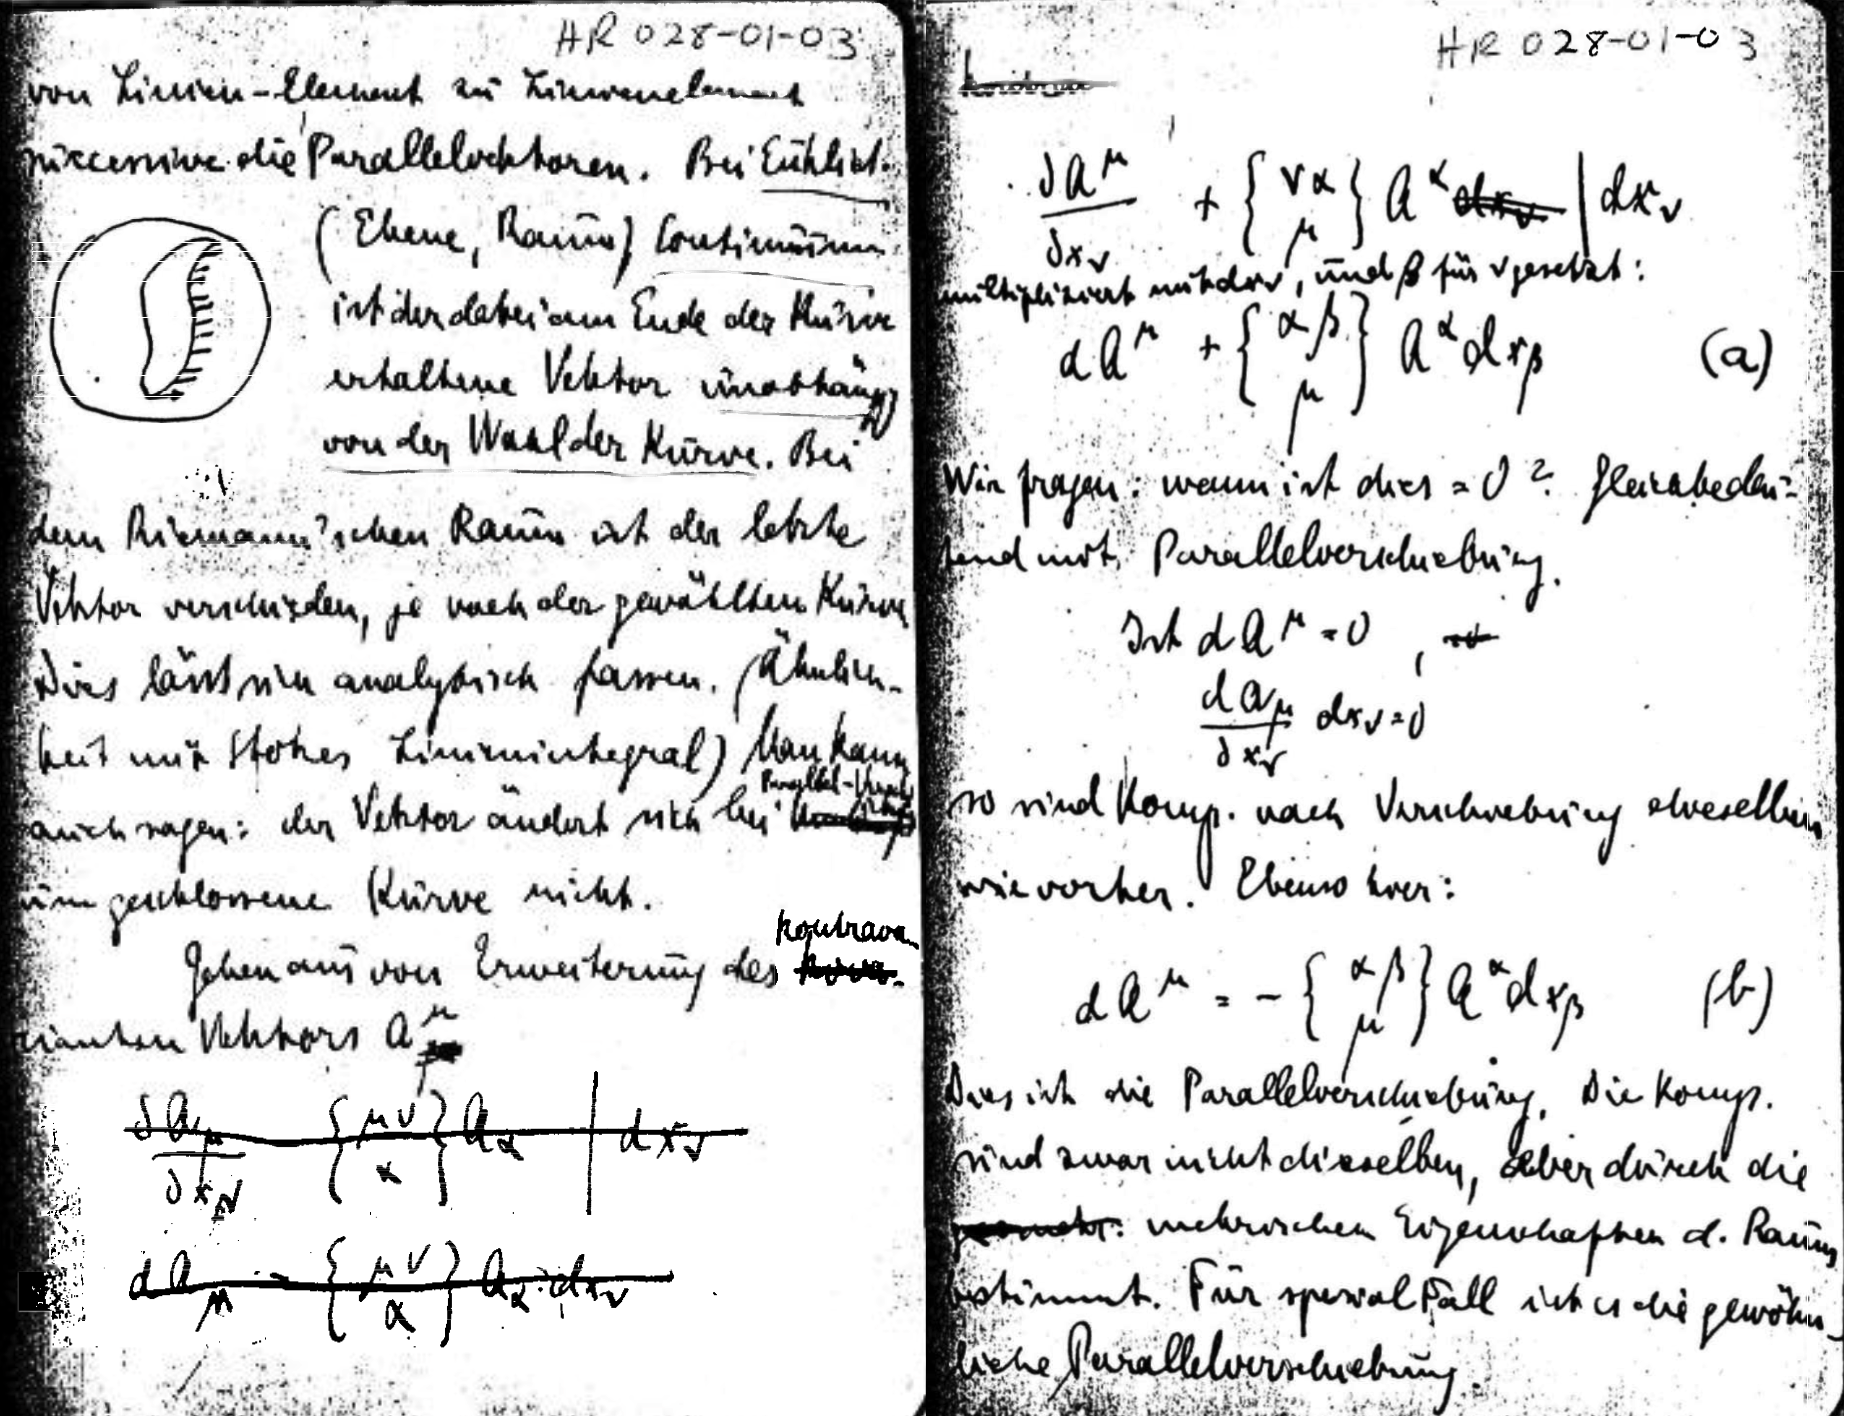
\includegraphics[scale=0.16, trim = 0mm 0mm 0mm 0mm, clip]{parallelverschiebungDOUB.png}
\caption{Reichenbach's student notes. Einstein introduces the notion of parallel transport of vectors}
\label{fig:parallel}
\end{center}
\end{figure}

%\q{It is not the geometrical interpretation of electricity} but a deeper assumption which lies at the basis of all these attempts; namely, \q{the assumption that the road to a simple conception, in the sense of a geometrical interpretation, is also the road to true relationships in nature} \rzlap{370}{517}.


Weyl's technical innovation in differential geometry played a fundamental role, not only in successive presentations of \gr \citep[see][45ff.]{Einstein1922}, but more prominently in the development of the \uftp. If one takes a symmetric \gmn as the fundamental variable, the Christoffel symbols are the only possible outcome. However, defining the displacement \Gtmn independently of the metric \gmn, the Riemannian connection $\Gtmn = - \christoffel{\mu}{\nu}{\tau}$ appears only as a special case that has been achieved by introducing a series of contingent conditions. Dropping some of these conditions results in additional mathematical degrees of freedom that could be used to accommodate the electromagnetic field alongside the gravitational field in a unified \scare{geometrical} description.

As is well known, \citet{Weyl1918b,Weyl1918a,Weyl1919a} was bothered by a conceptual asymmetry characterizing Riemannian geometry. The comparison of direction of vectors is path-dependent, whereas the comparison of their lengths remains distant-geometrical. To compensate for this \scare{mathematical injustice} \citep{Afriat2009}, Weyl introduced a more general affine connection that depends not only on the gravitational tensor \gmn but also on the four-vector \phin, which could be identified with the electromagnetic four-potential. However, since there was no analog of the equivalence principle, this identification was merely formal. However, in the absence of an analogon of the equivalence principle, the justification of such identification was merely formal\footnote{In \citets{Weyl1918a} theory the vector field \phin determines the change of length of vectors;  the curl of \phin is the length-curvature tensor \fmn, which satisfy satisfy an identity which \emph{looks a lot like} Maxwell-Minkowski equations in empty space. Thus, it was very suggestive to interpret \phin as the electromagnetic four-potential and its curl \fmn as the electromagnetic tensor}. Nevertheless, Weyl came to the conclusion that his theory offered a unified geometrization of both gravitational and electromagnetic phenomena, similar to how general relativity represented a geometrization of gravitational phenomena. Weyl did not hesitate to declare that \qt{Descartes' dream of a purely geometrical physics}{Der Traum des Descartes von einer rein geometrischen Physik} had been finally fulfilled \citep[263]{Weyl1919}.
%%


Einstein had repeatedly criticized Weyl's attempt\footnote{Einstein raised at least four objections against Weyl's theory: (1) the so-called \scare{measuring rod objection} (\german{Maßstab-Einwand}) \citep{Einstein1918b} is most famous. \WT predicts that the clocks' ticking rate should depend on the clocks' prehistory. However, the spectral lines of atoms used as clocks are well-defined; (2) the geodesic equation in Weyl's theory con­tains terms proportional to the vector potential \phin. Thus, the electromagnetic four-vector potential affects the motion of uncharged particles; (3) the representation of the Lagrangian is the mere sum of electromagnetic and gravitational components, thus \WT does not achieve a proper unification; (4) The field equations derived from this Lagrangian were of the fourth-order in the \gmn which, even in the absence of an electromagnetic field, did not reduce to the generally relativistic equations of gravitation, violating the correspondence principle}. Nevertheless, after corresponding with Theodore Kaluza in the spring of 1919\citep{Wuensch2005}\footnote{\lettercpae{Einstein}{Kaluza}{21}{4}{1919}[9][26]; \lettercpae{Einstein}{Kaluza}{28}{4}{1919}[9][30]; \lettercpae{Einstein}{Kaluza}{5}{5}{1919}[9][35]; \lettercpae{Einstein}{Kaluza}{14}{5}{1919}[9][40]; \lettercpae{Einstein}{Kaluza}{29}{5}{1919}[9][48])}, he had started to show increasing interest in the unification program \citep{Einstein1919a}. The question fell into the background after the success of the eclipse expedition was announced in November 1919 \citep{Dyson1920}. By the end of the year, Einstein was turned into an international celebrity, leaving him little time to work (\lettercpae{Einstein}{Fokker}{1}{12}{1919}[9][187], \lettercpae{Einstein}{Hopf}{2}{2}{1920}[9][295]). As a trained physicist with a doctorate in philosophy \citep{Reichenbach1916}, Reichenbach was uniquely positioned to engage with the philosophical implications of the theory. Through his attendance at Einstein's lectures, he had acquired a detailed technical knowledge of the new theory, surpassing that of most philosophers of his time. In February or March 1920, shortly after his move to Stuttgart, Reichenbach decided to make this topic the subject of his habilitation. According to his later recollections\footnote{These autobiographical notes \cite[044-06-23]{HR} were written in 1927}, in the preceding months, he had further worked on the theory \qt{also according to Weyl}{auch nach Weyl} \citep[044-06-23]{HR}---that is, probably studying Weyl's textbook \citetitle{Weyl1918} \citep{Weyl1918}. The Kapp-Pusch coup in \datemy{13}{3}{1920} rovided Reichenbach with a few days off from his job at the Huth radio industry  \citep[044-06-23]{HR}. This gave him the opportunity to work uninterrupted, and in just ten days, he completed an early draft of his habilitation. The manuscript was then typed and shown to Einstein and others. Thanks to the intervention of Arnold Berliner, the influential editor of \jt{Naturwisseschaften}, Reichenbach secured a publishing agreement with Springer \citep[044-06-23]{HR}.
%%

\subsection{Reichenbach's Habilitation and his Critique of Weyl Theory}


For the still Kantian Reichenbach, one of the main philosophical merits of the theory of relativity was the revelation of the physical character of geometry\footnote{Reichenbach's habilitation has recently attracted renewed attention \citep{Friedman2001}. Reichenbach borrowed from \citet{Schlick1918} the idea that physical knowledge is, ultimately (\emph{Zuordnung}), the process of relating an axiomatically defined mathematical structure to concrete empirical reality \citep{Padovani2009}. However, Reichenbach attempted to give this insight a \scare{Kantian} twist. According to Reichenbach, in a physical theory, besides the \scare{axioms of connections} (\german{Verknüpfungsaxiome}) encoding the mathematical structure of a theory, one needs a special class of physical principles, the \scare{axioms of coordination} (\german{Zuordnungsaxiome}), to ensure the univocal coordination of that structure to reality. For the young Reichenbach, the latter axioms are \apr because they are \scare{constitutive} of the object of a physical theory. However, they are not apodeictic or valid for all time. As is well known, Reichenbach would soon abandon the project of a constitutive but relativized \apr. However, he would firmly maintain the separation between the mathematical framework of a theory (the \scare{defined side}) and the way it relates to empirical reality (the \scare{undefined side}) as an essential feature of his philosophy \rhp{40}{42} as an essential feature of his philosophy}. The possibility of non-Euclidean geometries had already suggested that the Euclidean character of physical space could no longer be taken for granted \rhp{3}{3}. According to Reichenbach, \q{the theory of relativity embodies an entirely new idea} \rhp{3}{4}. \Rt claims that the theorems of Euclidean geometry do not apply to the physical space, that Euclidean geometry is simply \emph{false} \rhp{3}{4}. As a result, the development of \rt has made it necessary to differentiate between pure geometry as a formal system with no interpretation and applied geometry as an empirical theory of physical space \rhp{73}{76}. The propositions of pure geometry are neither true nor false in themselves. The question of the truth of physical geometry pertains to physics alone. In order to emphasize the importance of this philosophical achievement, almost incidentally, Reichenbach indicated Weyl's recent theory as a glaring example of how easy it was to slip into old habits. Weyl once again believed to have found a particular geometry that, for its intrinsic mathematical appeal, must have been \scare{true} for physical reality: \qt{In this way, the old mistake is repeated}{so begeht man nur den alten Fehler von neuem} \rhp{73}{76}.
%%%


Reichenbach's brief outline of \WT is sufficient to grasp the gist of his argument. As Reichenbach's put it, \qt{Weyl's generalization of the theory of relativity  \textelp{} abandons altogether the concept of a definite length for an infinitesimal measuring rod}{Weylschen Verallgemeinerung der Relativitätstheorie 22) entgegengehalten werden, bei der der Begriff einer feststehenden .Länge für einen unendlich kleinen Maßstab überhaupt aufgegeben wird} \rhp{73}{76}. In Euclidean geometry, a vector can be shifted parallel to itself along a closed curve so that, when brought back to the point of departure, it has the same direction and the same length. In the Einstein-Riemann geometry, it has the same length, but not the same direction. In \WT, it does not even retain the same length. As we have seen, in this way, in addition to the \scare{metric tensor} \gmn, a \scare{metric vector} $\phin$ is introduced that formally behave like the electromagnetic four-potential. Reichenbach conceded that \WT represented a possible generalization of Einstein's conception of \spti that, \qt{although not yet confirmed physically, is by no means impossible}{wenn auch physikalisch noch nicht bewiesen, doch auch keineswegs unmöglich ist} \rhp{76}{79}. 
%%%

Reichenbach seemed to have been aware of Einstein's main objection to Weyl's proposal \citep[see][]{Einstein1918b}. In general relativity, the length $ds$ of the time-like vector $dx_\nu$ is measured by a physical clock, e.g., by the crests of waves of radiation were emitted by an atom. If we maintain this interpretation, then \WT implies that \qt{the frequency of a clock is dependent upon its prehistory}{Nach der Weylschen Theorie ist die Frequenz einer Uhr von ihrer Vorgeschichte abhängig.} \rhp{77}{80}. It particular, it is affected by the electromagnetic potentials $\varphi_\nu$ it has encountered. Thus, two atomic clocks, at one place, will, in general, not tick at the same rate when they are separated brought back together. This result appears to contradict a vast amount of spectroscopic data that shows that all atoms of the same type have the same systems of stripes in their characteristic spectra independently of their past history. Reichenbach conceded to Weyl that these effects might \qt{compensate each other on the average}{daß sich diese Einflüsse im Durchschnitt ausgleichen,} \rhp{77}{80}. Thus, the fact that \qt{the frequency of a spectral line under otherwise equal conditions is the same on all celestial bodies}{Frequenz einer Spektrallinie bei sonst gleichen Umständen auf allen Himmelskörpern gleich ist, als Näherungen erklären} could be interpreted as an approximation, rather than a consequence of the Riemannian nature of space-time \rhp{77}{81}. According to Reichenbach, Weyl seems to imply that his non-Riemannian geometry must be true \emph{physically} because it is \emph{mathematically} superior to Riemannian geometry.
%%%%

As we have seen, in \WG, a vector moving around a closed loop would have the same length but a different direction, whereas in Riemannian geometry it would have different length and direction. Thus, \WG eliminated the last distant-geometrical treatment of Riemannian geometry. In this sense, \WG seems to be the most \scare{general geometry}, a purely infinitesimal geometry. As a consequence, there is no reason to assume that a more special geometry applies to reality from the outset. However, Reichenbach had already surmised that this generalization could be continued. In \WG, lengths can be compared at the same point in different directions but not at distant points. \qt{The next step in the generalization would be to assume that the vector changes its length upon turning around itself}{Die nächste Stufe der Verallgemeinerung wäre die, daß auch bei der Drehung um sich selbst der Vektor bereits seine Länge geändert hat} \rhp{76}{85}. Probably, more complicated generalizations could be thought of. \qt{Nothing may prevent our grandchildren from someday being confronted with a physics that has made the transition to a line element of the fourth degree}{Nichts könnte unsere Enkel davor schützen, dass sie eines Tages mit einer Physik konfrontiert werden, die zu einem Linienelement vom vierten Grad übergegangen ist} \rhp{76}{79}\footnote{$d s^{4}=g_{\mu \nu \sigma \tau} d x_{\mu} d x_{\nu} d x_{\sigma} d x_{\tau}$ instead of $d s^{2}=\gmn d x_{\mu} d x_{\nu}$ as in Riemannian geometry}. Thus, there is no \q{\scare{most general} geometry} that in and of itself must be physically true \rhp{76}{80}. No matter how far one pushes the level of mathematical abstraction, the \q{difference between physics and mathematics} \rhp{76}{80} cannot be erased; geometry alone can never be sufficient to establish the reality of physical space \rhp{76}{80}.
%%%

Reichenbach accused Weyl of neglecting the main philosophical lesson of \gr: the unbridgeable difference between physics and mathematics. According to Reichenbach, a mathematical axiom system is indifferent to the applicability of geometry, and it \q{never leads to principles of an \emph{empirical theory}} \rhp{73}{76}. On the other hand, only a physical theory can answer the question of the validity of a particular geometry for physical space \rhp{73}{76}.

\qt{[Thus] it is incorrect to conclude, like Weyl\footnote{In the 1919 edition of the \citetitle{Weyl1919}, Weyl included a presentation of his \uft. Thus, the \scare{Conclusion} of the book was characterized by even more inspired rhetoric: \q{physics and geometry coincide with each other} \citep[263]{Weyl1919}. The tendency of physicalizing geometry that prevailed among the leading protagonists of the 19th century from Gauss to Helmholtz seemed to be superseded by the project of geometrizing physics that ran from Clifford to Einstein: \q{geometry has not been physics but physics has become geometry} \citep[263]{Weyl1919}} and Haas\footnote{\cite{Haas1920}}, that mathematics and physics are but one discipline. The question concerning the \emph{validity} of the axioms for the physical world must be distinguished from that concerning \emph{possible} axiomatic systems. It is the merit of the theory of relativity that it has removed the question of the \emph{truth} of geometry from mathematics and relegated it to physics. If now, from a general geometry, theorems are derived and asserted to be a necessary foundation of physics, the old mistake is repeated. This objection must be made to Weyl's generalization of the theory of relativity \textelp{} Such a generalization is possible, but whether it is compatible with reality \myemph{does not depend on its significance for a general local geometry}. Therefore, Weyl's generalization must be investigated from the viewpoint of a physical theory, and only experience can be used for a critical analysis. Physics is not a \scare{geometrical necessity}; whoever asserts this returns to the pre-Kantian point of view where it was a necessity given by reason}{Ganz falsch ist es aber, wenn man daraus, wie z. B. Weyl und auch Haa.s tt), wieder den Schluß ziehen will, daß Mathematik und Physik zu einer einzigen Disziplin zusammenwachsen. Die Frage der Geltung von Axiomen für die Wirklichkeit und die Frage nach den möglichen Axiomen sind absolut zu trennen. Das ist ja gerade das Verdienst der Relativitätstheorie, daß sie die Frage der
Geltung der Geometrie aus der Mathematik fortge- nommen und der Physik überwiesen hat. Wenn man jetzt aus einer allgemeinen Geometrie wieder Sätze aufstellt und behauptet, daß sie Grundlage der PJ.iysik sein müßten, so begeht man nur den alten Fehler von neuem. Diest:r Einwand muß der Weylschen Verallgemeinerung der Relativitätstheorie 22) entgegengehalten werden, bei der der Begriff einer feststehenden .Länge für einen unendlich kleinen Maßstab überhaupt aufgegeben wird. Allerdings ist eine solche Verallgemeinerung möglich, aber ob sie mit der Wirklichkeit verträglich ist, hängt nicht von ihrer Bedeutung für eine allgemeine Nahegeometrie ab. Darum muß die Weylsche Verallgemeinerung vom Standpunkt einer physikalischen Theorie betrachtet werden, und ihre Kritik erfährt sie allein durch die Erfahrung. Die Physik ist eben ~eine „geometrische Notwendigkeit"; wer das behauptet, kehrt auf·den vorkantischen Standpunkt zu ück, wo sie eine vernunftgegebene Notwendigkeit war}[\rhp{73}{76}] 
%
To a certain extent, this objection contains the backbone of Reichenbach's criticism of the \uftp in the following decade. Weyl seems to have misunderstood the fundamental lesson of Einstein's theory. The question of the \q{\emph{validity} of axioms for the physical world} must be distinguished from that concerning \q{\emph{possible} the axiomatic systems} \rhp{73}{76}.
%%

It is true that it is \q{a characteristic of modern physics to represent all processes in terms of mathematical equations}, and, one might add, progressively more abstract mathematics. Still, \qt{the close connection between the two sciences must not blur their essential difference}{aber diese Berührung zweier Wissenschaften darf über deren grundsätzlichen Unterschied nicht hinwegtäuschen} \rhp{33}{34}. The truth of mathematical propositions depends upon internal relations among their terms, whereas the truth of physical propositions depends on the coordination (\german{Zuordnung}) to something external, on a connection with experience. \qt{This distinction is due to the difference in the objects of knowledge of the two sciences}{Es ist das Kennzeichen der modernen Physik, dass sie alle Vorgänge durch mathematische Gleichungen darstellt; aber diese Berührung zweier Wissenschaften darf über deren grundsätzlichen Unterschied nicht hinwegtäuschen} \rhp{33}{34}. The mathematical object of knowledge is uniquely determined by the axioms and definitions. These definitions have been called \qt{implicit definitions}{impliziten Definitionen} by \citet{Schlick1918}. They define one concept always through another concept without referring to external content \rhp{33}{36}. For this reason, mathematics is absolutely certain and \emph{necessary}. On the contrary, \q{the \emph{physical object} cannot be determined by axioms and definitions. It is a thing of the real world, not an object of the logical world of mathematics} \rhp{34}{37}. For this reason, physical knowledge always implies a certain degree of \emph{approximation}.

As is well-known, Reichenbach abandoned the Kantian framework in which the initial uncoupling of mathematics and physics was presented. However, he never abandoned the idea that a clear-cut division of labor between mathematical necessity and physical reality was of paramount epistemological importance. This separation was the irreversible conceptual shift that \rt had forced upon philosophy. On \datef{24}{6}{1920}, Einstein praised Reichenbach's \german{Habilitationschrift} in a letter to Schlick \lettercpaep{Einstein}{Schlick}{19}{4}{1920}[9][378]. A few days later, Reichenbach asked Einstein to dedicate the book to him, insisting on the philosophical significance of \rt:  \qt{very few among tenured philosophers have the faintest idea that your theory performed philosophical act and that your physical conceptions contain more philosophy than all the multivolume works by the epigones of the great Kant}{Philosophen eine Ahnung davon haben, dass mit Ihrer Theorie eine philosophische Tat getan ist, und dass in Ihren physikalischen Begriffsbildungen mehr Philosophie enthalten ist, als in allen vielbändigen Werken der Epigonen des grossen Kant} \lettercpaep{Reichenbach}{Einstein}{13}{6}{1920}[10][57]. Einstein conceded that the theory might have had philosophical relevance: \qt{The value of the th.\ of rel.\ for philosophy seems to me to be that it exposed the dubiousness of certain concepts that even in philosophy were recognized as small change \origins{Scheidemünzen}}{Der Wert der Rel.Th. für die Philosophie scheint mir der zu sein, dass sie die Zweifelhaftigkeit gewisser Begriffe dargethan hat, die auch in der Philosophie als Scheidemünzen anerkannt waren}  \lettercpaep{Einstein}{Reichenbach}{30}{6}{1920}[10][66]. Alleged \apr principles are like those parvenus that are ashamed of their humble origin and try to deny it: \qt{[c]oncepts are simply empty when they stop being firmly linked to experience}{Begriffe sind eben leer, wenn sie aufhören, mit Erlebnissen fest verkettet zu sein} \lettercpaep{Einstein}{Reichenbach}{30}{6}{1920}[10][66]. Einstein's remark, which Reichenbach would later quote in his published writing \citep[354]{Reichenbach1922a}, sealed a sort of philosophical alliance between them. Against Weyl's speculative style of doing physics, which reduced physical reality to geometrical necessity, Einstein defended a clear-cut separation between geometrical necessity and physical reality. However, as we shall see, this philosophical covenant would be broken less than a decade later.
%%%

%Reichenbach's booklet ultimately addressed the problem of the \scare{coordination} (\german{Zurordnung}) between mathematics and reality

%Sie gleichen Emporkömmlingen, die sich ihrer Abstammung schämen und sie verleugnen wollen

\subsection{The Reichenbach-Weyl Correspondence}
%EC an Hans Reichenbach, Hamburg 02. 07. 1920, 2 S., Pittsburgh. 285 EC an Hans Reichenbach, Hamburg 07. 07. 1920, 2 S., Pittsburgh.

Reichenbach's book was published in a timely manner a few months later in September 1920, on the occasion of the 86th \german{Versammlung der Gesellschaft Deutscher Naturforscher und Ärzte} in Bad Nauheim. This meeting was of fundamental importance in the history of \rt, not least because of the famous debate between Einstein and Philipp Lenard on general relativity \citep{Dongen2007}. At this meeting, Reichenbach met Weyl for the first time, who gave a talk on his unified theory \citep{Weyl1920}. Reichenbach may have attended the debate that followed Weyl's talk, in which Einstein rehearsed his objections against \WT and at the same time defended the possibility of a field theory of matter against Pauli's attacks. Einstein's famous lecture on \scare{geometry and experience} at the end of \datemy{27}{1}{1921} \citetitle{Einstein1921} was probably meant to address the epistemological issues that had emerged at Bad Nauheim \citep{Giovanelli2014a}. 
%%%

Reichenbach sent around copies of his \citetitle{Reichenbach1920a} \citep{Reichenbach1920a}. Schlick, who did not attend Bad Nauheim, received the book in those days. Writing to Einstein, he praised it but complained about his critique of conventionalism \lettercpaep{Schlick}{Einstein}{23}{9}{1920}. The five letters that Reichenbach exchanged with Schlick between October and November 1920\footnote{\letterhr{Schlick}{Reichenbach}{25}{9}{1920}[015-63-23]
\letterhr{Schlick}{Reichenbach}{26}{11}{1920}[015-63-22];
\letterhr{Schlick}{Reichenbach}{11}{12}{1920}[015-63-19]; \lettersa{Reichenbach}{Schlick}{29}{11}{1920}; \lettersa{Reichenbach}{Schlick}{10}{9}{1920}} turned out to be of fundamental importance in his intellectual biography, inducing him to abandon his early Kantianism in favor of a form conventionalism with empiricist traits\footnote{Reichenbach was confronted with Schlick's objection that his \scare{axioms of coordination} were nothing but \scare{conventions}. Reichenbach initially opposed some resistance. If the coordinating principles are fully arbitrary, he feared, geometry would be empirically meaningless. In Poincaré's conventionalism, Reichenbach missed a constraint in \qt{the arbitrariness of the principles \textelp{}, if the principles are combined}{daß die Willkürlichkeit der Prinzipien eingeschränkt ist, sowie man Prinzipien KOMBINIERT} \letterhr{Reichenbach}{Schlick}{26}{11}{1920}[015-63-22]. Einstein's famous lecture on \scare{geometry and experience} of the end \datemy{27}{1}{1921}, which was published a few months lter \citep{Einstein1921}, seemed to have tipped the scale in Schlick's favor. \citet{Reichenbach1922a} turned Einstein's $G+P$ formula into his $G + F$ formula, where $F$ is a \scare{metric} or universal force affecting all bodies in the same way. By setting $F=0$, geometry becomes empirically testable. Thus, Reichenbach could embrace conventionalism without accepting that the propositions of geometry are empirical meaningless}. Despite the rather severe criticisms he had expressed in the book \citep{Rynasiewicz2005}, Reichenbach must have sent a copy to Weyl as well. Weyl replied with some delay on \datemy{2}{2}{1921}. He did not appear to be upset by Reichenbach's objections and responded amicably to some issues that he felt \q{concerned less the philosophical than the physical} \letterhrp{Weyl}{Reichenbach}{2}{2}{1921}[015-68-04]. In particular, Weyl denied ever claiming that physics had been absorbed into mathematics:

\qt{It is certainly not true, as you say on p.\ 73, that, for me, mathematics (!!, e.g. theory of the $\zeta$-function?) and physics are growing together into a single discipline. I have claimed only that the \emph{concepts} in \emph{geometry} and field physics have come to coincide \textelp{} As for my extended theory of relativity, I cannot admit that the epistemological situation is in any way different from that of Einstein. \textelp{} \emph{Experience} is in no way anticipated by the assumption of that general metric; that the laws of nature, to which the propagation of action in the ether is bound, can be of such a nature that they do not allow any curvature. \textelp{} What I stand for is simply this: The integrability of length transfer (if it exists, but I don't think so, because I don't see the slightest dubious reason for it) does not lie in the nature of the metric medium, but can only be based on a special law of action\footnote{That is on the field equations of the theory which, in turn, can be derived from an \scare{action principle}}. If the historical development had been different, it seems that no one would have thought of considering the Riemannian case from the outset. As far as the notorious \scare{dependence on the previous history} is concerned, I probably expressed my opinion clearly enough in Nauheim}{ Was nıeine erweiterte Relativitätstlıeorie betrifft. so kann ich nicht zugeben, daß da erkenntnislogisch die Sache irgendwie anders liegt wie bei Einstein. \textelp{}  Der Erfahrung wird durch die Annahme jener allgemeiner Metrik in keiner Weise vorgegriffen; dass die Naturgesetze, an welche die Wirkungsausbreituug in Äther gebunden ist, können ja von solcher Art sein, daß sie keine Streıfkenkrümmung zulassen. \textelp{} Wofür ich allein eintrete, ist dies: Die Integrabilität der Strekken\"ubertraguug (wenn sie besteht, ich glaubs uielıt. denn ich sehe nicht den geriugsteu zwiugeudeu Grund dafür) liegt uielıt im Wesen des metrischen Mediumsm, sondern kann nur auf einem besonderen Wirkungsgesetz berulıen. Ware die historische Entwieklung anders verlaufien, so seheint nıir wåire uienıand darauf verfallen. von vorn- herein gerade nur den Rieuıauuselıeu Fall iu Erwåígımg zu zielıeu. - *Nas die berüchtigte “Abhšingigkeit von der Vorgeschichte" betrifft, so habe ieh darüber wohl nıeine Ansicht deutlieh gemıg in Naulıeinı ausgesprochen. An der 4. Aufl. wird Sie wahrscheinlich vor al- lenı nıeine veränderte Stellımgnalnue zum Problem der Materie i}[\letterhrp{Weyl}{Reichenbach}{2}{2}{1921}[015-68-04]]
%
In Bad Nauheim, Weyl presented a now well-known speculative explanation for the discrepancy between the behavior of \scare{ideal} and \scare{real} rods. Essentially, Weyl suggested that the atoms used as clocks might not \emph{retain} their size when transported, but rather \emph{adjust} it every time to some constant field quantity, which he identified with the constant radius of the spherical curvature of every three-dimensional slice of the world \citep{Weyl1920a}. As a result of this adjustment mechanism, the geometry read off from the behavior of material bodies would appear different from the actual geometry of \spti, due to the \scare{distortion} caused by the adjustment. In 1921, the \scare{pivotal year} for unified field theories \citep[ch.\ 4]{Vizgin1994}, Weyl (followed to some extent by \cite{Eddington1921,Eddington1921a}) expanded his strategy of \scare{doubling of the geometry}, including the real \scare{aether geometry} and the \scare{body geometry} distorted by the adjustment mechanism\footnote{A different variation of this strategy of \scare{doubling the geometry} was suggested by \citet{Eddington1921} at about the same time. He considered non-Riemannian geometries as mere \scare{graphical representations} that might serve to organize different theories into a common mathematical framework. The \q{natural geometry} remains exactly Riemannian \citep{Eddington1921}}, in three papers intended for different audiences, published in February \citep{Weyl1921a}, May \citep{Weyl1921d} and July \citep{Weyl1921e}. In the July paper, Weyl also addressed Reichenbach's criticism publicly:

\qt{From different sides\footnote{The reference is to \cite{Reichenbach1920a} and \cite{Freundlich1920} who, however, refers to \cite{Haas1920}}, it has been argued against my theory that it would attempt to demonstrate in a purely speculative way something \emph{a priori} about matters on which only experience can actually decide. This is a misunderstanding. Of course from the epistemological principle \origins{aus dem erkenntnistheoretischen Prinzip} of the relativity of magnitude does not follow that the \scare{tract} displacement \origins{Streckenübertragung} through \scare{congruent displacement} \origins{durch kongruente Verpflanzung} is not integrable; from that principle that no \emph{fact} can be derived. The principle only teaches that the integrability \emph{per se} must not be retained, but, if it is realized, it must be understood as the \myemph{outflow \origins{Ausfluß} of a law of nature}}{3. Von verschiedenen Seiten?) ist gegen meine Theorie eingewendet worden, daß in ihr aus reiner Spekulation Dinge a priori demonstriert würden, über .welche nur die Erfahrung entscheiden kann. Das is ein Mißverständnis. Aus dem erkenntnistheoretischen Prinzip von der Relativität der Größe folgt natürlich nicht, daß die Streckenübertragung durch kongruente Verpflanzung nicht integrabel ist; es folgt aus ihm überkaupt keine-Tatsache. Es lehrt nur, daß Integrabilität an sich nicht zu bestehen braucht, sondern, wenn sie stattfindet, als Ausfluß eines Naturgesetzes verstanden werden muß}[\citep[475; last emphasis mine]{Weyl1921b}]
%
As Weyl explains in this passage, he never claimed that his geometry entails in its mathematical structure alone the \apr justification of its physical truth. On the contrary, he questioned the supposed \apr status of the assumption that the comparison of lengths is path-independent. For this reason, Weyl did not deny the well-established empirical fact that the spectral lines of two atoms of the same chemical substance, placed identically in the same conditions, remain unaffected by their prehistory. However, he mantains that, in principle, the physical behavior of atoms does not have anything to do with the abstract notion of parallel transport of vectors\footnote{\label{pauli}In September 1921, \citets{Pauli1921} encyclopedia article on relativity theory was published as part of the fifth volume of the \bt{Enzyklopädie der Mathematischen Wissenschaften}. In the chapter dedicated to \WT, Pauli suggested that Weyl provided two different versions of the theory. In its first version, \WT sought to make predictions on the behavior of \rac, just like Einstein's theory. From this point of view, the theory is empirically meanigful, but inadequate because of the existence of atoms with sharp spectral lines. Later, Weyl renounced this interpretation. The ideal process of the congruent displacement vectors has nothing to do with the real behavior of \rac \citeptra[763]{Pauli1921}[196]{Pauli1958}. However, in this way, the theory furnishes only \q{formal, and not physical evidence for a connection between \textins{the} world metric and electricity} \citeptra[763]{Pauli1921}[196]{Pauli1958}. In this form, Pauli argues, the theory loses its \q{convincing power \origins{\"{U}berzeugungskraft}} \citeptra[763]{Pauli1921}[196]{Pauli1958}}. Einstein assumed as an empirical fact that the ratio of the wave lengths of two spectral lines is a  physical constant that can be used to normalize the $ds$. Weyl, on the contrary, claims that the wave lengths of two spectral lines are always a multiple of a certain field quantity of dimension of a length that can be used to normalize the $ds$. 
%%%

\subsection{The Weyl-Reichenbach Appeasement}

\hide{Im Sept. 1921 trug ich schon den ersten Bericht \"uber die Axiomatik auf dem Physikertag in .lena vor.3 Ich hatte damals gro§en Erfolg; aber niemand ist damals auf den Gedanken gekommen, mich in eine angemessene Stelle zu berufen. Ich blieb in Stuttgart sitzen. Niederschrift und Ausbau im Winter 1921 /22.}  \hide{Niederschrift und Ausbau im Winter 1921/22. Das alte MS wurde völlig umgestoßen. Genauere Behandlung der allg. Th. im Aug.-Spt. 1922. Vortrag darüber in Leipzig, Sept. 1922.}

Weyl's paper referencing Reichenbach appeared at the beginning of September \citep{Weyl1921e}. A few weeks later, Reichenbach and Weyl met again in Jena on the occasion of the first  \german{Deutsche Physiker- und Mathematikertag}, the first national scientific meeting held independently from the meetings of the \textit{Gesellschaft Deutscher Naturforscher und Ärzte}. Weyl gave a talk in which he tried to provide a mathematical justification for the quadratic or Pythagorean nature of the metric \citep{Weyl1921f}. Reichenbach presented a report of his work on the axiomatization of relativity \citep{Reichenbach1921d}. This report is the first written testimony of the development of Reichenbach's philosophy after the Schlick correspondence. Reichenbach suggested that, in a physical theory, one should distinguish the \emph{axioms} as an empirical proposition about light rays, \rac\etc and the \emph{definitions} that establish the conceptual framework of the theory \lettercpaep{Reichenbach}{Einstein}{5}{12}{1921}[12][266]. After the paper came out by the end of the year \citep{Reichenbach1921d}, Reichenbach must have sent a copy to Weyl in a missing letter of \datef{8}{1}{1922}. He might have included a personal retraction of his criticisms. However, the letter, which is no longer extant, reached Weyl only months later \letterhrp{Weyl}{Reichenbach}{3}{3}{1922}[015-68-03], since he was in Barcelona, where he was giving his Catalonian Lectures \citep{Weyl1923}.

However, Reichenbach soon issued a public retraction. During that time, he was working on a lengthy review article about philosophical interpretations of relativity that he finished in the Spring of 1922. In March, Erwin Freundlich sent the proofs of the paper to Einstein \lettercpaep{Freundlich}{Einstein}{24}{3}{1922}[13][109], who generally concurred with Reichenbach's analysis \lettercpaep{Einstein}{Reichenbach}{27}{3}{1922}[13][119]. The paper reviewed the most significant philosophical interpretations of relativity. However, it also included a last section on Weyl's \uft: \q{One cannot conclude an exposition of relativistic philosophy without considering the important extension that Weyl bestowed on the problem of space three years ago}{Man darf eine Darstellung der relativistischen Philosophie nicht abschließen, ohne der wichtigen Erweiterung zu gedenken, die vor 3 Jahren Weyl dem Raumproblem zuteil werden ließ} \citep[365]{Reichenbach1922a}, Reichenbach commented.

Reichenbach now appears to be fully committed to conventionalism. The choice between Euclidean and non-Euclidean geometries is based on a \emph{convention} about which rods should be considered rigid \citep[366]{Reichenbach1922a}. This convention is arbitrary but can be fixed by postulating that metrical forces should be eliminated \citep{Reichenbach1922}. However, both Euclidean and non-Euclidean geometries implicitly assume the validity of an axiom based on an \emph{empirical fact}: rods of equal length in one place can be obtained in another place, regardless of the prehistory of each rod. If this were not the case, a different definition of the unit of length would have to be given for every point in space. Reichenbach referred to this tacit assumption as the \qt{axiom of the Riemann class}{Axiom der Riemannklasse} \citep[366]{Reichenbach1922a}. Weyl's merit is to have demonstrated that this axiom, although quite natural, is not necessary and can be challenged.

From this point of view, what Weyl achieved is a purely mathematical result: \qt{Weyl's great discovery is that he uncovered a more general type of manifold, of which Riemann's space is only a special case}{Die grosse Entdeckung Weyls besteht darin, daß er einen allgemeineren Mannigfaltigkeitstypus aufdeckte, von dem auch der Riemannsche Raum nur ein Spezialfall ist} \citep[365]{Reichenbach1922a}. The fact that he tried to follow this path, regardless of its empirical correctness, was a \q{genial advance \origins{genialer Vorstoß}} in the philosophical foundation of the relations between geometry and physics \citep[367f.]{Reichenbach1921}. Concerning the application of this mathematical apparatus to reality, Reichenbach embraces what might be called the two-theory interpretation\footnote{Reichenbach might have been inspired by \citet{Pauli1921}. However, his name is not mentioned}:
%%%
\begin{W}
\item\label{W1} In \WG, as in Riemannian geometry, the length of vectors  $l^2=\gmn A^\nu A^\mu$ can be compared at the same point in different directions. Weyl dropped the assumption that $l$ remains unchanged under parallel transport at a distant point. If a vector of length $l$ is displaced from $x_\nu$ to $x_\nu+dx_\nu$, it will, in general, have a new length $l+dl$, so that $dl/l=\phin dx_\nu$. \q{The change in scale is measured by 4 quantities $\varphi_{\mu}$ forming a vector field}. As Reichenbach pointed out, \qt{this procedure is a purely \ls{mathematical} discovery}{Dieses Verfahren ist zunächst eine rein \ls{mathematische} Entdeckung} \citep[366]{Reichenbach1922a}, and as such is neither true nor false. It acquires a physical meaning if one coordinates the length $l$ as readings of some physical measuring instruments. In \gr, the length $ds$ of the time-like vector $dx_\nu$ is measured by a clock, \eg, the spectral lines of an atomic clock. Weyl considered natural to maintain this interpretation, so that it is \qt{still possible to measure also in this case}{auch in diesem Fall überhaupt noch zu »messen«} \citep[366]{Reichenbach1922a}. However, the existence of atoms with the same spectral lines shows that clocks, even in the presence of the electromagnetic field, behave differently than predicted by \WT. Thus, it turned out that this axiom \qt{is quite well fulfilled in reality, so the first way of generalization seems unsuitable. The latter was therefore rejected by Weyl}{Es zeigt sich allerdings, daß dieses Axiom in der Wirklichkeit recht gut erfüllt ist, so daß der erste Weg der Verallgemeinerung ungeeignet erscheint. Er wird deshalb von Weyl abgelehnt}  \citep[366]{Reichenbach1922a}.

\item\label{W2} Weyl adopted a different strategy. He \qt{defines an ideal process of scale transfer, which, however, has nothing to do with the behavior of real scales}{definiert einen ideellen Prozeß der Maßstabs-Uebertragung, der jedoch mit dem Verhalten realer Maßstäbe nichts zu tun hat}  \citep[367]{Reichenbach1922a}. He needs this \qt{transplantation process}{Verpflanzungsprozeß} only because, he  \qt{he wants to identify the vector field \phin with the electromagnetic potential}{er das Vektorfeld \phin mit dem elektromagnetischen Potential identifizieren will}, like in \gr the \gmn were identified with the gravitational potentials \citep[367]{Reichenbach1922a}. Once one has individuated the basic geometrical field-quantities, the next step is to find the field equations \qt{then obvious forms for the most general physical equations arise}{dann naheliegende Formen für die allgemeinsten physikalischen Gleichungen entstehen} via \qt{the \scare{action principle} \origins{Wirkungsprinzip}}{(für das »Wirkungsprinzip«}  \citep[367]{Reichenbach1922a}---a variational principle applied to the invariant integral $\int \mathfrak{W} d x$ for a specific Lagrangian $\mathfrak{W}$. According to Reichenbach, however, in this way the \qt{theory loses its convincing character \origins{überzeugenden Charakter} and comes dangerously close to a mathematical formalism}{Theorie ihren überzeugenden Charakter und kommt einem mathematischen Formalismus bedenklich nahe, der um eleganter mathematischer Prinzipien willen die Physik unnötig kompliziert; und aus diesem Gedanken heraus wird die Weylsche Theorie von Physikern (besonders auch von Einstein) sehr zurückhaltend betrachtet.}\footnote{This choice of words is similar to that of Pauli, who claimed that \WT in the second form lost his \emph{Uberzeugunggkraft} \citeptra[763]{Pauli1921}[196]{Pauli1958}}  \citep[367]{Reichenbach1922a}. For this reason, according to Reichenbach, \qt{\WT is viewed very cautiously by physicists (especially by Einstein)}{aus diesem Gedanken heraus wird die Weylsche Theorie von Physikern (besonders auch von Einstein) sehr zurückhaltend betrachtet}  \citep[367]{Reichenbach1922a}.
\end{W}
%
Ultimately, Reichenbach seems to imply that both strategies led to a dead end. From the point of view of \ref{W1}, Weyl's infinitesimal geometry is physically inadequate; from the point of view of \ref{W2}, it is physically empty. Nevertheless, Reichenbach conceded that his objection against \WT in his 1920 booklet missed the point. Neither \ref{W1} nor \ref{W2} can be considered attempts to prove \apr that Weyl's non-Riemannian geometry must be true for reality because it is mathematically preferable as a truly infinitesimal geometry:

\qt{However, I have to retract my earlier objection [\cite[73]{Reichenbach1920}] that Weyl wants to \ls{deduce} physics from reason, after Weyl has cleared up this misunderstanding [\cite[475]{Weyl1921b}]. Weyl takes issue with the fact that Einstein simply accepts the unequivocal transferability of the standards. He does not wish to dispute the Riemann-class axiom for natural standards, but only to demand that the validity of this axiom, since it is not \ls{logically} necessary, should be understood as \scare{a consequence of a law of nature}. I can only agree with Weyl's demand; it is the importance of mathematics that they are. I can only agree with Weyl's demand; it is the importance of mathematics that, in uncovering more general possibilities, it marks the special facts of experience \ls{as special} and thus preserves physics from naivity \origins{Simplizität}. Admittedly, Weyl succeeds in explaining the unambiguous transferability of natural standards only very imperfectly. But the fact that Weyl tried to go this way, regardless of the empirical correctness of his theory, remains an ingenious advance towards the philosophical foundation of physics}{Ich muß jedoch meinen früher erhobenen Einwand (47, S. 73), daß Weyl die Physik aus der Vernunft deduzieren will, zurücknehmen, nachdem Weyl dieses Mißverständnis aufgeklärt hat (72, S. 475). Weyl stößt sich daran, daß bei Einstein die eindeutige Uebertragbarkeit der Maßstäbe einfach hingenommen wird. Er will nicht das Axiom der Riemannklasse für natürliche Maßstäbe bestreiten, sondern nur fordern, daß die Geltung dieses Axioms, da es nicht logisch notwendig ist, als »Ausfluß eines Naturgesetzes verstanden werde«. Ich kann dieser Forderung Weyls nur zustimmen; es ist die Bedeutung der Mathematik, daß sie mit dem Aufdecken allgemeinerer Möglichkeiten die speziellen Tatbestände der Erfahrung als speziell kennzeich net und SO die Physik vor Simplizität bewahrt. Freilich gelingt Weyl die Erklärung der eindeutigen Uebertragbarkeit natürlicher Maßstäbe nur sehr unvollkommen 1). Aber daß Weyl diesen Weg zu gehen versucht, bleibt unabhängig von der empirischen Richtigkeit seiner Theorie ein genialer Vorstoß zur philosophischen Grundlegung der Physik}[\citep[367f.]{Reichenbach1922a}]
%
Weyl's point was not that the axiom of the Riemann class is necessarily false for \apr reasons, but on the contrary, that it is not \apr true as previously assumed. The fact that two measuring rods placed next to each other are of the same length regardless of their location cannot be a coincidence; it demands an explanation. Weyl's explanation of the apparent Riemannian behavior of \qt{through the adaptation to the radius of \scare{curvature of the world}{Krümmungsradius der Welt}}{durch Einstellung der Maßstäbe auf den Krümmungsradius der Welt} \citep[368\fn{1}]{Reichenbach1922a} only poses a problem rather than providing an answer. The problem would only be solved by developing a proper theory of matter. However, even if this theory could be provided, Reichenbach, like Einstein, found the idea of deducing the Riemannian behavior of real clocks from a theory based on the non-Riemannian behavior of geometrical lengths awkward. In this way, the \qt{congruent transplantation \textelp{} remains physically empty}{stellung« nichts zu tun mit seiner kongruenten Verpflanzung, so dass diese physikalisch leer bleibt} \citep[368\fn{1}]{Reichenbach1922a}. If the non-Riemannian congruent transplantation of vectors must be, Reichenbach argues, then the real rods should behave better in a non-Riemannian way.

Thus, Reichenbach concluded that the main achievement of Weyl was mathematical and not physical. As has often happened in the past, mathematics enlarges the range of possibilities from which physicists can choose. However, this process is far from concluded with Weyl's rather special affine connection:

\qt{The \ls{philosophical} significance of Weyl's discovery is that it proved that the problem of space could not be considered concluded even with Riemann's concept of space. If contemporary epistemology attempted to update Kant's transcendental aesthetics by asserting that the geometry of experience must, in any case, possess a Riemannian structure, it would be refuted by \WT. That \WG is at least \ls{possible} for reality cannot be denied. Furthermore, it should not be assumed that \WT has reached the highest level of generality. As \citet{Einstein1921c} has demonstrated, Weyl's requirement of the relativity of magnitude can also be satisfied without using Weyl's measurement method. In addition, \citet{Eddington1921} developed a further generalization of which Weyl's space \origins{Raumklasse} is merely a special case. Eddington's space \origins{Raumklasse} is again included as a special case in a more general one discovered by \citet{Einstein1921c}. The merit of Schouten's theory is that it provides the conditions under which a space \origins{Raumklasse} can be considered the most general; these are very general conditions, such as differentiability and the like. Nevertheless, it must be acknowledged that there is no absolutely most general space. The history of the mathematical problem of space should instruct epistemology never to make such sweeping claims. There are no most general concepts}{Die \ls{philosophische}  Bedeutung der Weylschen Entdeckung besteht deshalb darin, daß sie bewiesen hat, daß ein Abschluß des Raumproblems auch mit dem Riemannschen Raumbegriff nicht gegeben ist. Wollte also die Erkenntnistheorie heutP- die Behauptung der transzendentalen Aesthetik Kants dahin erweitern, daß die Geometrie der Erfahrung auf jeden Fall wenigstens von Riemannscher Struktur sein muß, so wird sie durch die Weylsche Theorie daran zurückgehalten. Denn daß der Weylsche Raum wenigstens für die Wirklichkeit  \ls{möglich} ist, läßt sich nicht bestreiten. Man darf nicht einmal glauben, daß mit der Weylschen Theorie nun die höchste Stufe der Allgemeinheit erklommen sei. Einstein hat gezeigt (14), daß man die Weylsche Forderung der Relativität der Größe auch befriedigen kann, ohne von dem Weylschen Meßverfahren Gebrauch zu machen. Danach wurde von Eddington (15) wieder eine Verallgemeinerung entwickelt, von der die Weylsche Raumklasse nur ein Spezialfall ist, und die Eddingtonsche Raumklasse ist wieder als Spezialfall in eine allgemeinere eingegangen, die von Schouten (63) gefunden wurde. Der Vorzug der Schoutenschen Theorie besteht darin, daß hier die Bedingungen angegeben werden, unter welchen die entwickelte Raumklasse die allgemeinste ist; es sind sehr allgemeine Bedingungen, wie Differenzierbarkeit und ähnliches. Aber eine schlechthin allgemeinste Raumklasse gibt es natürlich nicht; und die Geschichte des mathematischen Raumproblems mag der Erkenntnistheorie eine Lehre sein, niemals schlechthin allgemeine Behauptungen aufzustellen. Es gibt keine allgemeinsten Begriffe}[\citep[368\fn{1}]{Reichenbach1922a}]
%
This passage essentially repeats Reichenbach's argument in his habilitation: there is nothing special in \WG. However, it also shows that, in the meantime, Reichenbach had closely followed the development of the \uftp. He was familiar with \citets{Einstein1921c} \scare{conformal} theory, in which distances can be compared only at a single point with light rays, but the comparison at distant points with transportable rods was not defined. Reichenbach was also familiar with \citets{Eddington1921} purely affine approach in which lengths go vectors cannot be compared even not at the same place in different directions. Moreover, it is quite impressive that he was even acquainted with \citets{Schouten1922} recent systematic classification of connections. Thus, Reichenbach was already aware that, in principle, also the natural assumption of the symmetry of the \Gtmn could be dropped. In general, relaxing the constraints on the symmetry of the connection and the relationship between the connection and the metric could open up many possibilities for incorporating the electromagnetic field into the geometrical structure of spacetime. 
%%%

In Reichenbach's view, physicists should be completely free to choose among all these mathematical possibilities. However, mathematics alone cannot provide a criterion for choosing which possibility is realized in nature. Mathematics is the science of possibility, while physics is the science of reality. Once a choice has been made, it is essential to coordinate the chosen structure with the behavior of various idealized physical entities used as probes. Only in this way can the choice of the geometrical structure of spacetime be tested experimentally. E.g., in general relativity, the claim that in the presence of real gravitational fields, the \spti geometry is non-flat can be confirmed or disconfirmed by \rach measurements. Weyl initially followed the same epistemological model  \ref{W1}. In the presence of the electromagnetic field, \rac should behave in a non-Riemannian way. However, this prediction turned out to be empirically inadequate. As a response, Weyl embraced \ref{W2}. He embraced a sort of conspiratorial distortion of all measuring instruments. However, in doing so, he deprived the geometrical setting of any empirical content.

Weyl disagreed with Reichenbach's historical reconstruction, but for reasons that reveal a completely different frame of mind. In a letter to Reichenbach, written when the latter's review article was already in press, Weyl confessed that he actually never abandoned \ref{W1} in favor of \ref{W2}. As a matter of fact, he never adopted \ref{W1} in the first place. As he wrote to Reichenbach: \qt{I never gave up the plan to identify rigid rods with my transplantation, because I've never had that plan}{Den Plan, starre Maßstäbe mit meiner Verpflanzımg zu identifizieren, habe ich aufgegeben. weil ich ihm nie gehabt habe}; on the contrary, \qt{I was surprised when I said that physicists had interpreted that into my words}{ich war überrascht, als ich salı, daß Physiker das in meine Worte hineininterpretiert hatten} \letterhrp{Weyl}{Reichenbach}{20}{05}{1922}[015-68-02]. The atoms that we use as clocks are physical systems like any other and do not have in principle any privileged relation with the abstract mathematical behavior of vectors. It is the theory that decides whether we should use them as reliable clocks or not. Generally, the physical interpretation of the theory's mathematical structure in terms of the behavior of idealized physical entities, like \rac, can only be provisional. Ultimately, one has to find the field equations governing that structure and require that solutions to these equations exist exhibiting the postulated behavior of \rac. This reasoning applies to Einstein and \WT: \qt{Einstein has to show that from the dynamics of the rigid body, it follows that the rod always has the same length, measured in his $ds$. Similarly, I have to show that the rod has always had the same length normalized $ds$ normalized by $R = const$}{Genau, wie  Einstein zeigen muß, daß aus der Dynamik des starren Körpers heraus ein solches Verhalten folgt, daß der Maßstab immer dieselbe Länge hat, gemessen in seinem $ds$, so muß ich zeigen, daß er immer das gleiche durch $R = const$ normierte $ds$ hat} \letterhrp{Weyl}{Reichenbach}{20}{05}{1922}[015-68-02]. In both cases, the behavior of rods and clocks comes out as a byproduct of the theory\footnote{In such a theory, the unit of length would be defined as certain number of spacing between the atoms of a cubic crystal system; each of atom, in turn, consists of electrons and protons arranged according to a specific law. A specific solution to the field equations must provide information about all the details of this arrangement. Something similar can be said for the unit of time that correspond to the vibrations of an atom}. However, in \WT, the Riemannian behavior of \rac that came out at the end contradicts the non-Riemannian length connection on which the theory was based (see, \eg, \lettercpae{Du Pasquier}{Einstein}{13}{12}{1921}[12][379]).

\section{Geometrization: The Reichenbach-Einstein Correspondence (1926--1927)}
\label{geometrization}
%
Up to this point, Reichenbach had good reasons to believe that his criticisms of Weyl's approach broadly agreed with Einstein's point of view. Thus, Einstein continued to express skepticism towards Weyl's \scare{Hegelian} approach to physics  \lettercpaep{Einstein}{Zangger}{1}{1}{1921}[12][5]. He lamented a lack of \q{\emph{physical} clues} for these attempts at unification \lettercpaep{Einstein}{Lorentz}{30}{6}{1921}[12][163] that were therefore still too speculative (\lettercpae{Einstein}{Weyl}{6}{6}{1922}[13][219]; \lettercpae{Einstein}{Zangger}{18}{6}{22}[13][241]). However, the situation changed by the end of 1922, when Einstein, during a trip to Japan, realized that Eddington's theory had potentialities that had not been fully exploited. 

On board the ship, he jotted down a five-page manuscript dated January 1923 from Singapore \CPAEp{13}{417}. Curiously, the third, fourth, and fifth pages were written on the reverse side of Reichenbach's Jena talk typescript \citep{Reichenbach1921}. \citet{Eddington1921} had extended Weyl's approach by using only the coefficients of an affine connection \Gtmn, rather than metrical quantities \gmn and \phin, as fundamental variables. In this context, vectors' lengths are not even comparable at the same place; thus, in Einstein's view, the theory avoided Weyl's inconsistency of having geometrical lengths behaving differently from real numbers. On \datemy{15}{2}{1923}, Planck presented Einstein's attempt to derive a set of field equations to the Prussian Academy of Sciences \citep{Einstein1923c}. After returning to Berlin, Einstein published two further papers on the same approach in May \cite{Einstein1923c,Einstein1923e}.
%%%

In \datemy{2}{5}{1923}, Reichenbach requested a copy of Einstein's paper \q{on Eddington's extension \origins{Erweiterung}} \citep{Einstein1923c} \letteraeap{Reichenbach}{Einstein}{2}{5}{1923}[20 080]. He did not comment on Einstein's unification attempt at this point\footnote{As one might infer from Reichenbach's later writings, his point of view might have been similar to that of Pauli. In a long letter to Eddington in September 1923, Pauli insisted that a good theory should start with \qt{the definition of the field quantities used, and how these quantities can be measured}{einer Definition der verwendeten Feldgrößen beginnen muss, die angibt, wie diese Größen gemessen werden können} \letterpaulip{Pauli}{Eddington}{23}{9}{1923}[45]. One of the great achievements of relativity theory was that the coefficients \gmn could be measured with \rac. Pauli explained that Weyl attempted to pursue this strategy again but then abandoned this approach \letterpaulip{Pauli}{Eddington}{23}{9}{1923}[45]. In this way, he produced what Eddington had rightly called a \scare{graphical representation} of the two fields in unified formalism, but not a \scare{natural geometry} found experimentally as in general relativity \citep[see][197]{Eddington1923}. Similarly, in Einstein-Eddington new theory \qt{[t]he quantities [\Gtmn] cannot be measured directly}{Die Größen [\Gtmn] können nicht direkt gemessen, sondern müssen aus den direkt gemessenen Größen erst durch komplizierte Rechenoperationen gewonnen werden} \letterpaulip{Pauli}{Eddington}{23}{9}{1923}[45]. The measurable quantities \gmn and \fmn can be calculated from the \Gtmn only through complicated calculations. Thus, not only we do not have a \qt{\scare{natural geometry} but also not a \scare{natural theory}}{dann haben wir nicht nur keine \scare{natural geometry}, sondern auch keine \scare{natural theory}} \letterpaulip{Pauli}{Eddington}{23}{9}{1923}[45]}. In his correspondence with Einstein, Reichenbach was concerned with the more mundane matter of finding a publisher for his work on the axiomatization of \sr that he had just finished (\letteraea{Reichenbach}{Einstein}{19}{4}{1923}[20 079], \letteraea{Reichenbach}{Einstein}{2}{5}{1923}[20 080], \letteraea{Einstein}{Reichenbach}{9}{6}{1923}[20 081], \letteraea{Reichenbach}{Einstein}{10}{7}{1923}[20 082]). Due to a lack of funding, Reichenbach managed to publish the book only a year later, in March 1924. With the \citetitle{Reichenbach1924} \citet{Reichenbach1924}, Reichenbach's philosophy started to assume a more recognizable contour. In particular, Reichenbach introduced, for the first time, his celebrated distinction between \q{conceptual definitions} used in mathematics and \q{coordinate definitions} used in physics, which relate the concept of a theory to a \q{piece \originsg{Ding} of reality} \citeptra[5]{Reichenbach1924}[8]{Reichenbach1969}. There is little doubt that Reichenbach believed this epistemological model was Einsteinian in spirit. However, at about that time, Einstein explicitly confessed that he had changed his mind on the topic \citepp[1692]{Einstein1924}[see][]{Giovanelli2014a}. In particular, he denied that every individual concept of a theory should receive a measurement-operational justification \citep[1691]{Einstein1924}. Ultimately, only geometry and physics together could be compared with experience \citep[19]{Einstein1926}, a claim that seems to have a different meaning than Reichenbach had initially surmised.

The \citetitle{Reichenbach1924} \citep{Reichenbach1924} received a lukewarm reception from philosophers, who probably found the book overly technical. However, it was \citets{Weyl1924} negative review that dealt a hard blow to Reichenbach and ended their previously amicable relationship. Reichenbach felt that Weyl had used his authority as a mathematician to attack his \scare{empiricist} reading of relativity \citep{Reichenbach1925}. What was worse, Reichenbach must have sensed that Weyl's \scare{geometrical} reading of relativity had taken over relativistic research. Einstein's latest works seemed to reveal that he had also fallen under its spell\footnote{As Weyl himself ironically remarked, Einstein undertook \q{the same purely speculative paths which \textins{he was} earlier always protesting against} (\lettercpae{Weyl}{Einstein}{18}{5}{23}[13][30]; cf.\ \letter{Weyl}{Seelig}{19}{5}{1952}, cit.\ in \cite[274f.]{Seelig1960})}. Unsurprisingly, Reichenbach might have felt it necessary to make a case for a different interpretation of \rt in a more accessible form. At about the same time, he started work on a two-volume book with the ambitious title \bt{Philosophie der exakten Naturerkenntnis}. Only the first volume on space and time will be published. He wrote the first chapters in March 1925 \citep[044-06-25]{HR}.

During those same months, despite Max Planck's support, Reichenbach struggled to obtain his \german{Umhabilitation}\footnote{The process of obtaining the \latin{venia legendi} at another university} from Stuttgart to Berlin to be appointed to a newly created chair of natural philosophy \citep{Hecht1982}. Reichenbach had been attacked for his pacifist positions during the war, but after the situation seemed to have turned for the better, he started working more consistently on his book project in October 1925. He interrupted the drafting of the manuscript to follow the emerging quantum revolution at the turn of 1926 and must have started again a few months later: \qt{March-April 1926 \WT was worked on, and the peculiar solution of \S49 was found. The entire \Ap was also written at that time. (Correspondence with Einstein)}{März-April 1926 wurde die Weylsche Theorie bearbeitet u. die eigentümliche Lösung des § 49 gefunden. Auch wurde damals der ganze Anhang geschrieben. (Korrespondenz mit Einstein)} \citep[044-06-25]{HR}. The correspondence with Einstein mentioned in this passage has been preserved. It reveals Reichenbach's concerns with Einstein's style of doing physics becoming progressively more speculative, forsaking the solid empirical foundation of his old theory of gravitation.
%%%

\subsection{Reichenbach's Geometrization of the Electromagnetic Field}
%
%npublished opening lecture for the course on the theory of relativity in Argentina
During a trip to South America in 1925, Einstein became interested in the rationalistic and realistic reading of relativity proposed by \'Emile \citetp{Meyerson1925} \CPAE{14}{455, 6; \datedm{12}{3}{1925}} who could provide a more adequate philosophical support for the search of a \uft than Schlick's or Reichenbach's \scare{positivism} \cite{Giovanelli2018a}. However, he also realized that the Weyl-Eddington-Schouten line had dried up (\CPAE{14}{455, 9; \datedm{17}{3}{1925}}). Returning from South America, he embraced what he considered a new approach. He introduced non-symmetric \Gtmn and the \gmn to be treated as independent fields in the variation. The antisymmetric part of the \gmn was the natural candidate for representing the electromagnetic field, at least for infinitely small fields. The physical test depended, as usual, on the construction of exact regular solutions corresponding to elementary particles. The paper was published in \datemy{1}{9}{1925} with the ambitious title \citetitle{Einstein1925a}  \citep{Einstein1925a}. However, by that time, Einstein seemed to have already lost his confidence in that approach and moved on.

At the turn of the year, after working on the new quantum mechanics, Reichenbach must have read Einstein's new paper. On \datef{16}{3}{1926}, Reichenbach sent a letter to Einstein in which, after discussing his academic misfortunes, he made some critical remarks \citep{Einstein1925a}. Reichenbach was quite skeptical of the viability of Einstein's current style of doing physics:

\qt{I have read your last work on the extended Rel.\ Th.\footnote{\cite{Einstein1925a}} more closely, but I still can't get rid of a sense of artificiality that characterizes all these attempts since Weyl. The idea, in itself very deep, to ground the affine connection independently of the metric on the \Gtmn alone, serves only as a calculation crutch here in order to obtain differential equations for the \gmn and the \phin and the modifications of the Maxwell equations which allow the electron as a solution. If it worked, it would, of course, be a great success; have you achieved something along these lines with Grommer? However, the whole thing does not have the beautiful convincing power \origins{Ueberzeugungskraft} of the connection between gravitation and the metric based on the equivalence principle of the previous theory}{Ich habe jetzt Ihre letzte Arbeit zur erweiterten Rel. Th. genauer gelesen, aber ich kann auch da das Gefühl des Künstlichen nicht los werden, das allen diesen Versuchen seit Weyl anhaftet. Die an sich doch sehr tiefe Idee, den affinen Zusammenhang unabhängig von dem metrischen zu begründen allein auf die $\Gamma^{i}_kl$ dient doch schließlich nur als Rechenknüppel, um Differentialgleichungen für die $g_{ik}$ und $\varphi_ik$ zu bekommen und solche Abänderungen der Maxwellschen Gleichungen zu bekommen, die das Elektron als Lösung zulassen. Wenn das geht, ist es natürlich ein großer Erfolg; haben Sie eigentlich mit Herrn Grommer etwas in dieser Richtung errichtet? Aber die ganze Sache hat doch nicht die schöne Ueberzeugungskraft, wie die auf das Aequivalenz-Prinzip gestützte Verknüpfung von Gravitation und Metrik in der früheren Theorie}[\lettercpaep{Reichenbach}{Einstein}{16}{3}{1926}[15][224]]
%
Reichenbach's objections are quite sensible and not dissimilar to those of professional physicists\footnote{In a review of the German translation \citep{Eddington1925} of Eddington's relativity textbook \citep{Eddington1923} that came out a few weeks later, \citet{Pauli1926} expressed similar concerns. Without the equivalence principle, the entire geometrization program appeared to Pauli unjustified: \qt{An attempt at an analogous geometrical interpretation of the electromagnetic field faces the difficulty that there is no empirical fact corresponding to the equality of heavy and inert mass, which would make such an interpretation appear \scare{natural}}{Einem Versuch ether anatogen geometrischen Deutung des elektromagnetischen Fetdes steht nun die Schwierigkeit entgegen, dab bier keine tier Gleichheit yon schwerer und träger Masse entsprechende Erfahrungstatsache vorliegt, die eine solche Deutung als "natürlich" erscheinen lassen warde} \citep{Pauli1926}. The solution was to avoid any connection between geometry and the behavior of \rac. However, in this way, one could at most produce what Eddington called a \scare{graphical representation}. According to Pauli, similar objections could be raised against Einstein's last work \citep{Einstein1925}}. In general relativity, the choice of the \gmn as fundamental variables is anchored in the principle of equivalence. The latter justified the double meaning of the \gmn, as determining the behavior of \rac, as well as the gravitational field. On the contrary, Einstein's new theory introduces the non-symmetric affine connection \Gtmn independently of the metric \gmn without giving to these field variables any physical motivation. The separate variation of the metric and connection was nothing more than a \scare{calculation device} to find the desired field equations. Only in hindsight, for formal reasons, the symmetric part of the \gmn was identified with the gravitational field and antisymmetric with the electromagnetic field. In this form, the theory has little he \scare{convincing power} (\german{Überzeugungskraft})----the same expression that \citet[367]{Reichenbach1921} had used for characterizing \WT in his second form. Reichenbach would have been ready to retract his criticism, if Einstein's theory delivered the \scare{electron}. This concession, however, barely hides his skepticism that a field theory of matter was a credible possibility.

Einstein replied on \datedm{20}{3}{1926}  that he agreed with Reichenbach's \scare{$\Gamma$-Kritik}: \qt{I have absolutely lost hope of going any further using these formal ways}{Ich habe jetzt jede Hoffnung aufgegeben, auf diesem formalen Wege weiter zu kommen}; \q{without some real new thought} he continued, \qt{it simply does not work}{Ohne einen wirklich neuen Gedanken geht es nicht} \lettercpaep{Einstein}{Reichenbach}{20}{3}{26}[15][230]. Einstein's reaction reflects his disillusion with the attempts with an approach based on the generalization of Riemannian geometry by weakening the relations by \gmn and \Gtmn. He would have probably been less ready to embrace the implications of Reichenbach's $\Gamma$-critique, the requirement that the operation of parallel displacement of vectors should receive a \scare{coordinative definition} from the outset. At any rate, Reichenbach took the opportunity of Einstein's positive reaction, and on \datef{31}{3}{1926} sent him a note \citep{Reichenbach1926f},  in which he developed the $\Gamma$-critique in detail \lettercpaep{Reichenbach}{Einstein}{24}{3}{1926}[15][235].

\begin{figure}
\begin{center}
 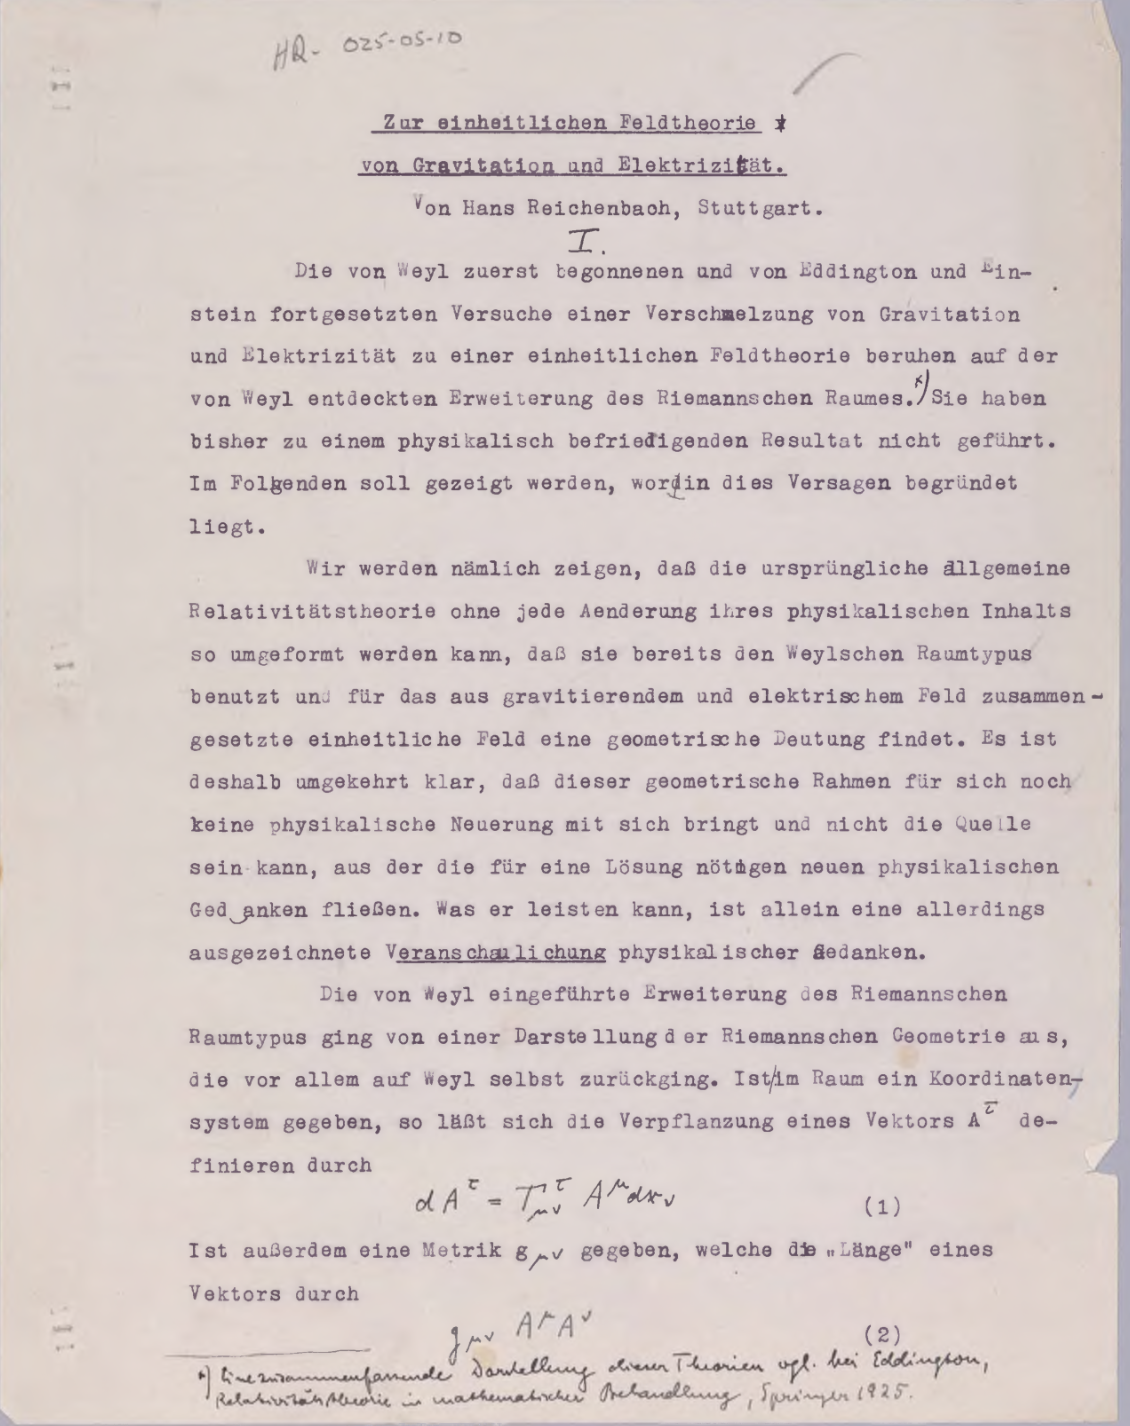
\includegraphics[scale=0.4, trim = 0mm 0mm 0mm 0mm, clip]{1926ReichenbachNote}
 \caption{Reichenbach's note on the geometrization of the electromagnetic field}
\end{center}
\end{figure}

A point-by-point commentary of Reichenbach's note has been provided elsewhere \citep{Giovanelli2016d}. Reichenbach introduced a non-symmetric \Gtmn to define an operation of displacement expressing the effect of both the gravitational and electromagnetic fields. In Riemannian geometry, the straightest lines are the shortest between two points. If the connection is non-symmetric, the straightest lines generally do not coincide with the shortest (or, more precisely, the lines of extremal length). Charged mass points of unit mass move (or their velocity four-vector is parallel-transported) along the straightest lines, and uncharged particles move on the straightest lines that are at the same time the shortest ones (or rather, the line of extremal length) \citep{Reichenbach1926f}.

Einstein was not impressed \lettercpaep{Einstein}{Reichenbach}{31}{3}{1926}[15][239].  Thus, Reichenbach rushed to point out that Einstein had misunderstood the spirit of the typescript. As Reichenbach explained, he was working on a book on the philosophy of space and time, and thereby he \qt{wondered what the geometrical presentation of electricity actually means}{Dabei überlegte ich mir, was die geometrische Darstellung der Elektrizität eigentlich bedeutet} \lettercpaep{Reichenbach}{Einstein}{4}{4}{1926}[15][244].  Reichenbach wanted to challenge the idea that geometrizing a field is per se a useful heuristic strategy: \q{If one succeeds in establishing unified field equations that admit the electron as a solution, this would be \myemph{something new}.} \lettercpaep{Reichenbach}{Einstein}{4}{4}{1926}[15][244]. To this purpose, however, the  Maxwell and Einstein field equations needed to be  \emph{modified}: \q{This is the problem on which you are working and of course also what Weyl and Eddington meant} \lettercpaep{Reichenbach}{Einstein}{4}{4}{1926}[15][244]. However, the geometrical representation of electricity in itself does not lead to this goal. \q{It can at most be an aid \origins{Hilfsmittel} to guessing the right equations}; it might be that \q{what looks most simple from the standpoint of Weyl geometry also happens to be correct. But this would be only a coincidence\label{zufall}} \lettercpaep{Reichenbach}{Einstein}{4}{4}{1926}[15][244]. 

With his theory, Reichenbach \q{wanted to turn against the notion that something had already been gained with the geometrical presentation of electricity} \lettercpaep{Reichenbach}{Einstein}{4}{4}{1926}[15][244]. In comparison with Eddington or Einstein's last proposals, Reichenbach insisted, his approach had even the advantage \qt{that \emph{the operation of displacement possesses a physical realization \textins{Realisierung}}}{Diese Umschreibung hat aber vor anderen geometrischen Darstellungen den Vorteil, daß sie für die Verschiebungsoperation eine physikalische Realisierung besitzt} \lettercpaep{Reichenbach}{Einstein}{4}{4}{1926}[15][244], namely, the velocity-vector of charged mass particles. In this way, the notion of the straightest and shortest lines is physically meaningful. For this reason, in Reichenbach's view, his geometrization was comparable to that provided by \gr. Nevertheless, differently from Einstein's theory of gravitation, Reichenbach's theory did not lead to any new physical prediction. Thus, Reichenbach concluded, a successful geometrization does not necessarily lead to a successful physical theory. 

Although Einstein probably continued to find the technical details of Reichenbach's attempt questionable, his philosophical point clearly resonated with Einstein:

\qt{You are completely right. It is incorrect to believe that \scare{geometrization} means something essential. It is instead a mnemonic device \origins{Eselsbrücke} to find numerical laws. If one combines geometrical representations \origins{Vorstellungen} with a theory, it is an inessential, private issue. What is essential in Weyl is that he subjected the formulas, beyond the invariance with respect to \textins{coordinate} transformation, to a new condition (\scare{gauge invariance})\footnote{That is, invariance by the substitution of $g_{ik}$ with $\lambda g_{ik}$ where $\lambda$ is an arbitrary smooth function of position \citep[c\f][468]{Weyl1918}. Weyl introduced the expression \scare{gauge invariance} (\german{Eichinvarianz}) in \cite[114]{Weyl1919a}}. However, this advantage is neutralized again, since one has to go to equations of the 4. order%
%
\footnote{Cf.~\cite[477]{Weyl1918}. Einstein regarded this as one of the major shortcomings of \WT; see \letter{Einstein}{Besso}{20}{8}{1918}[\VD{8b}{604}][CPAE], \letter{Einstein}{Hilbert}{9}{6}{1919}[\VD{9}{58}][CPAE]},%
%
which means a significant increase of arbitrariness}{Lieber Herr Reichenbach\\ Sie haben vollständig recht. Es ist verkehrt zu glauben, dass die \scare{Geometrisierung} etwas Wesentliches bedeutet Es ist mir eine Art Eselsbrücke zur Auffindung numerischer Gesetze. Ob man dann mit einer Theorie \scare{geometrische} Vorstellungen verbindet, ist unwesentliche Privatsache. Das Wesentliche bei Weyl liegt darin, dass er die Formeln neben der Invarianz bezüglich Transformationen einer neuen Bedingung (\scare{Eichinvarianz}) unterwirft. Dieser Vorteil wird aber wieder neutralisiert dadurch, dass man zu Gleichungen 4. Ordnung übergehen muss, was ein beträchtliches Wachsen der Willkür bedeutet.\\Mit besten Grüssen \\Ihr A. Einstein}[\lettercpaep{Reichenbach}{Einstein}{8}{4}{1926}[15][249]]
%
Einstein seems to endorse Reichenbach's claim that a \scare{geometrization} is not an essential achievement of general relativity. However, it is worth noticing that Einstein goes beyond Reichenbach and claims that the very notion of \scare{geometry} is meaningless \citep{Lehmkuhl2014}. The \gmn, \Gtmn\etc. are ultimately multi-components mathematical objects characterized by their transformation properties under change of coordinates. There is nothing \scare{geometrical} about those quantities. Thus, Einstein's point is only superficially similar to that of Reichenbach. Einstein declared that the difference between geometry and the rest of mathematics was inessential. On the contrary, as we shall see, Reichenbach intended to show that the difference between geometry and physics was essential. Einstein's argument was meant to provide support to the \uftp. Against those that believed that the geometrization program could not be extended beyond the gravitational field, he could argue that geometrization has never been the issue in the first place\footnote{\citets{Pauli1926} review of the German translation of \citet{Eddington1925} is a typical example of this type of criticism}. Reichenbach's argument, on the other hand, was an attack on the belief that geometrization by itself would lead to physical results.

\subsection{The \Ap to the \PRZL}

Strengthened by Einstein's endorsement, Reichenbach presented the note in Stuttgart at the regional meeting of the German Physical Society on \datem{26}{5}{1926} \citep{Reichenbach1926d}. In the following months, he must have further work on the manuscript of his book and by the end of the year, he could write to Schlick that \qt{[t]he first volume that deals with space and time [was] finished}{der erste Band der Raum und Zeit behandelt, ist fertig} \letterp{Reichenbach}{Schlick}{6}{12}{1926}[][SN]\label{RZL1926}. Reichenbach hoped to publish the book in the forthcoming Springer series \scare{Schriften zur wissenschaftlichen Weltauffassung} directed by Schlick and Philipp Frank. However, Springer rejected the book as being too long. By July, Reichenbach could announce to Schlick that he had reached a publication arrangement with de Gruyter \letterp{Reichenbach}{Schlick}{2}{7}{1927}[][SN]. The publisher agreed to publish only the first volume under the title \citetitle{Reichenbach1928}. According to \Reich's recollections, the manuscript was not changed significantly after February 1927\hide{Das MS war seit Febr. 1927 nicht mehr nennenswert geändert worden} \citep[044-06-25]{HR}. The drafts were finished in September, and the preface was dated October 1927. The note that Einstein had sent to Einstein in the Spring of 1926 became, with few changes, the \S49 of an extended \Ap dedicated to the modern development of differential geometry and the problem of the geometrical interpretation of electricity. If read with the inclusion of the \Ap\footnote{The \Ap was not included in the English translation \cite{Reichenbach1958}}, the \PRZL appears as a much more complex book. It was not only as a defense of a \scare{conventionalist} reading of the foundations of geometry, as it is usually claimed; it was at the same time an attack on the widespread interpretation of \gr as a \scare{geometrization} of the gravitational field \rzl{294}{256}.

The \Ap to the \PRZL was simply a continuation of the line of argument that was only partially developed in the last chapter of the book. \q{The geometrical interpretation of gravitation}, Reichenbach wrote using an effective analogy, \q{is merely the visual cloak in which the factual assertion} encoded by the equivalence principles \q{is dressed} \rzlap{354}{493}. The cloak might be conceived as an inextensible network of \rac tailored to the body of the gravitational field. However, \q{[i]t would be a mistake to confuse the cloak with the body which it covers; rather, we may infer the shape of the body from the shape of the cloak which it wears. After all, only the body is the object of interest in physics} \rzlap{354}{493}. The fact that a Euclidean cloak, so to speak, does not fit the body of a real gravitational field allows knowing something new about the shape of the body, that is, to make the \emph{new} predictions about the behavior of free-falling mass particles, light rays, clocks\etc. Unfortunately, according to Reichenbach, recent relativistic research seemed to have confused the cloak for the body itself. \q{The great success, which Einstein had attained with his geometrical interpretation of gravitation} led many \q{to believe that similar success might be obtained from a geometrical interpretation of electricity} \rzlap{352}{491}. 

After the physics community accepted \gr as a theory of gravitation, the search for a suitable geometrical cloak that could cover the naked body of the electromagnetic field began. The separation of the \scare{operation of displacement of vectors} \Gtmn from the operation of comparison of length at a distance \gmn gave physicists new mathematical degrees of freedoms that could be exploited to accommodate the electromagnetic field alongside the gravitational field. \q{However, the fundamental fact which would correspond to the principle of equivalence is lacking} \rzlap{354}{493}. Thus, physicists needed to proceed through trial and error in the search for suitable geometrical-field variables. Initially, attempts were made to identify these geometrical structures with the \scare{true} the geometry of \spti. The latter was supposed to be endowed with a more general affine structure. To give this claim empirical content, Weyl initially provided a \q{realization of the process of displacement} \Gtmn in terms of the behavior of \rac. Weyl's project failed because \rac did not behave as predicted by the theory in the presence of an electromagnetic field. Weyl found \q{a cloak} in which he could dress the new theory, but did not have \q{the body that this new cloak would fit} \rzlap{353}{493}.

Despite the failure of Weyl's project, physicists did not abandon the geometrization program. Instead, they came to the conclusion that \q{such \scare{tangible} \origins{handgreifliche} realizations does not lead to the desired field equations} \rzlap{371}{517}. Thus, theories were proposed by \q{Weyl, Eddington and Einstein} that \q{renounced such a realization of the process of displacement} \rzlap{371}{517}. The geometrical structures chosen, such as the \Gtmn, \phin, the \Gtmn, and \gmn, did not have any physical meaning from the outset, i.e., the values of the coefficients of those \scare{structures} were not the results of measurements. Einstein himself \q{has devised several new formulations in which the geometrical interpretation is reduced to the role of a mathematical tool \origins{Rechenhilfsmittels}} \rzlap{369}{516}. The key was to identify appropriate dynamical variables that could be used to construct the correct action and obtain the desired equations. However, since the fundamental variables did not have any physical meaning, the resulting field equations could not be directly compared with experience, as in the case of \gr.

The field equations could be confronted with reality only by integrating them in the hope that they yield a solution for the \scare{electron}. On the one hand, in Maxwell's \ed the cohesion of the electron's charge has always been attributed to a \scare{foreign force}; namely, the force of cohesion that keeps the Coulomb forces from exploding. Einstein's theory of gravitation, on the other hand, does not imply any effect of gravitation on charge and cannot, therefore, yield the cohesive force. To find a solution to the problem of matter, Maxwell's and Einstein's field equations should be valid to \q{a high degree of approximation} to recover the success of previous theories in the case of weak fields; yet they should be \q{changed, because, otherwise, they would never give us the electron as a solution} \rzlap{370}{517}. Physicists have to guess what kind of change has to be put forward. Without an analogon of the equivalence principle, they have become convinced that, \q{\textins{i}n this \scare{guessing}, the geometrical interpretation of electricity is supposed to be the guide} \rzlap{371}{517}. The point of departure in this approach was \q{the (unwritten) assumption that whatever looks \emph{simple} and \emph{natural} from the viewpoint of the geometrical interpretation will lead to the desired changes in the equations of the field} \rzlap{370}{517}. 

\q{The many ruins along this road}, Reichenbach pointed out, should have suggested physicists \q{that solutions should be sought in an entirely different direction} \rzlap{370}{517}. Why did they persist? Reichenbach quite perceptively grasped their psychological motivation: \q{It is not the geometrical interpretation of electricity} but a deeper assumption which lies at the basis of all these attempts; namely, \q{the assumption that the road to a simple conception, in the sense of a geometrical interpretation, is also the road to true relationships in nature} \rzlap{370}{517}. The geometrical interpretation provided by \gr was based on a physical hypothesis, the equivalence principle, which, in turn, was based on an empirical fact, the identity of gravitational and inertial mass. The \uftp is based on a different \emph{physical hypothesis} of a more speculative nature, the hypothesis that the world is geometrically simple. Indeed, by reading papers on the \uft, one is struck by the fact that they are full of expressions like \scare{most natural assumption}, \scare{simplest invariant}\etc \rzlap{370}{517}.

Needless to say, Reichenbach considered the idea that the \scare{simplicity} of a geometrical setting could have a bearing on its physical truth to be the consequence of a severe conceptual mistake \rzlap{372}{519}. He conceded that the final decision on whether the \uftp is worth pursuing \q{must be left to the physicist, whose physical instinct provides the sole illumination} \rzlap{372}{519}. Ultimately, the scientists' \q{physical instinct}, their deep conviction that the world is mathematically simple, pertains to the realm of the logic of discovery and thus lies outside the competence of epistemology. However, Reichenbach made no secret of the fact that he hoped to protect scientists from \q{the sirens' enchantment \origins{Sirenenzauber} of a unified field theory} by denouncing, once again, physicists' never-ending temptation to blur mathematics and physics \citep[373]{Reichenbach1928}.

\section{Unification: Reichenbach-Einstein Correspondence (1929--1930)}
\label{unification}
%
In October 1927, Reichenbach moved back to Berlin, where he took the position of an \q{unofficial associate professor} \citep{Hecht1982}. At about the same time, Einstein read the manuscript of the \PRZL \lettercpaep{Einstein}{Elsa Einstein}{23}{10}{1927}[16][34]. Soon after that, he wrote a short book review. Einstein was quite perceptive noting the two themes that Reichenbach had treated in the \Ap: \begin{inparaenum}[(1)] \item \qt{In the \Ap, the foundation of the Weyl-Eddington theory is treated in a clear way and in particular the delicate question of the \myemph{coordination} of these theories to reality}{In einem Anhang wird dann noch die Grundlage der Weyl-Eddingtonschen Theorien in klarer Weise dargestellt und insbesondere die heikle Frage der Zuordnung dieser Theorien zu der Wirklichkeit behandelt} \citep[20\me]{Einstein1928d}. As we have seen, Reichenbach had insisted that, as in any other theory, also in \uft based on the affine connection is a fundamental variable, one should give physical meaning to the operation of displacement from the outset. Einstein did not comment further on this issue since he realized that this requirement was too strict. However, Einstein seemed to fully agree with the second point made by Reichenbach: \item In the \Ap, \qt{in my opinion quite rightly---it is argued that the claim that general relativity is an attempt to \emph{reduce physics to geometry} is unfounded}{In diesem Kap., sowie in den vorangehende wird~--~meiner Ansicht nach mit vollem Recht~--~die Haltlosigkeit der These behauptet, nach welcher die Relativitätstheorie ein Versuch sei, die Physik auf Geometrie zurückzuführen} \citep[20\me]{Einstein1928d}. \end{inparaenum} As we have seen, Reichenbach and Einstein had already discussed this topic in a private correspondence less than two years earlier (\cref{geometrization}). 

At about the same time, Einstein published a more extensive review of Meyerson's \citetitle{Meyerson1925} \citep{Meyerson1925} in the \citejournal{Einstein1928b}. The review reveals how Einstein's perspective had become quite different from that of Reichenbach on both issues. Einstein embraced Meyerson's rationalist philosophy, insisting on the deductive-speculative nature of physics' enterprise, implicitly disavowing the operational-empirical rhetoric that seemed to have dominated his early philosophical pronouncements. However, Einstein strongly disagreed with Meyerson's insistence that Weyl's and Eddington's theories were the crowning moment of a long process of geometrization of physics. He insisted again that geometry in this context is \qt{\myemph{devoid of meaning}}{le terme \scare{g\`eom\`etrique} employ\`e dans cet ordre d'id\`ees est enti\`erement vide de sens} \citep[165\me]{Einstein1928b}. He clarified, however, that the essential point of the theories of Weyl and Eddington was not to geometrize the electromagnetic field, but to \q{represent gravitation and electromagnetic \myemph{under a unified point of view}, whereas beforehand these fields entered the theory as logically independent structures} \citep[165\me]{Einstein1928b}. Einstein's further attempts at \uft in the immediately following months reveal more clearly the reasons behind his philosophical turnabout \cite{Giovanelli2018a}

During a period of illness in the spring of 1928, Einstein came up with a new proposal for a \uft. On \datef{7}{6}{1928} Planck presented to the Prussian Academy a note on a \scare{Riemannian Geometry, Maintaining the Concept of Distant Parallelism} \citep{Einstein19281}---a flat space-time that is nonetheless non-Euclidean since the connection \Gtmn is non-symmetrical. He introduced a new formalism based on the concept of $n$-\german{Bein} (or $n$-legs), $n$ unit orthogonal vectors representing a local coordinate system attached to a point of an $n$ dimensional continuum. Vectors at distant points are considered as equal and parallel if they have the same local coordinates with respect to their \nbein. The \vbein-field \hbein defines both the metric tensor \gmn and the electromagnetic four-potential $\fm$. Its sixteen components can be considered as the fundamental dynamical variables of the theory. The question arises as to the field equations that determine the \vbein-field. In his second paper, submitted on \datedm{14}{6}{1928}, Einstein derived the field equations for the \vbein-field using a variational principle \citep{Einstein19282}.

A few months later, after the paper had been published, Reichenbach was able to prepare a typewritten note \citep{Reichenbach1928a} containing some comments which he sent to Einstein for feedback:
 
\qt{Dear Herr Einstein,\\ I did some serious thinking on your work on the field theory and I found that the geometrical construction can be presented better in a different form. I send you the ms. enclosed. Concerning the physical application of your work, frankly speaking, it did not convince me much. \myemph{If geometrical interpretation must be, then I found my approach simply more beautiful, in which the straightest line at least means something.} Or do you have further expectations for your new work?}{Lieber Herr Einstein, \\ Ich habe mir Ihre neuen Arbeiten zur Feldtheorie durch Kopf gehen lassen und gefunden, dass man die geometrische Aufbau besser in anderer Form darstelle kann. Ich schicke Ihnen einliegend des Ms. Was die physikalische Anwendung betrifft, so hat mich Ihre Arbeit, offen gesagt, wenig überzeugt. \myemph{Wenn es nun einmal geometrische Deutung sein muss, so finde ich schlechthin meinen Ansatz schöner, bei dem die geradesten Linien wenigstens etwas bedeuten}. Oder sollten Sie doch noch Aussichten in Ihren neuen Ansatz sehen?}[\letter{Reichenbach}{Einstein}{17}{10}{1928}][20-92\me][EA]
%
"n this passage, Reichenbach makes two unrelated points, which, however, appear to form a single two-pronged argument. In the note he sent to Einstein. \citet{Reichenbach1928b} demonstrated that---if one lets aside from the \nbein formalism---Einstein's new geometrical settings could be easily inserted into the Weyl--Eddington--Schouten lineage, as a special case of metric space in which the connection is flat, but non-symmetric\footnote{Starting from a general non-symmetric affine connection \Gtmn and imposing the condition that the length of vectors does not change under parallel transport, one can obtain Einstein and Riemann spaces through the \q{exchangeability of the specializations} \citep[5]{Reichenbach1928a}. By imposing that the Riemann tensor vanishes, one obtains Einstein space, while imposing that the connection is symmetric yields Riemannian space}. If so, Reichenbach could raise the same objection he had raised against Einstein's previous theories. 

\begin{figure}
%{L}{0.5\textwidth}
\centering
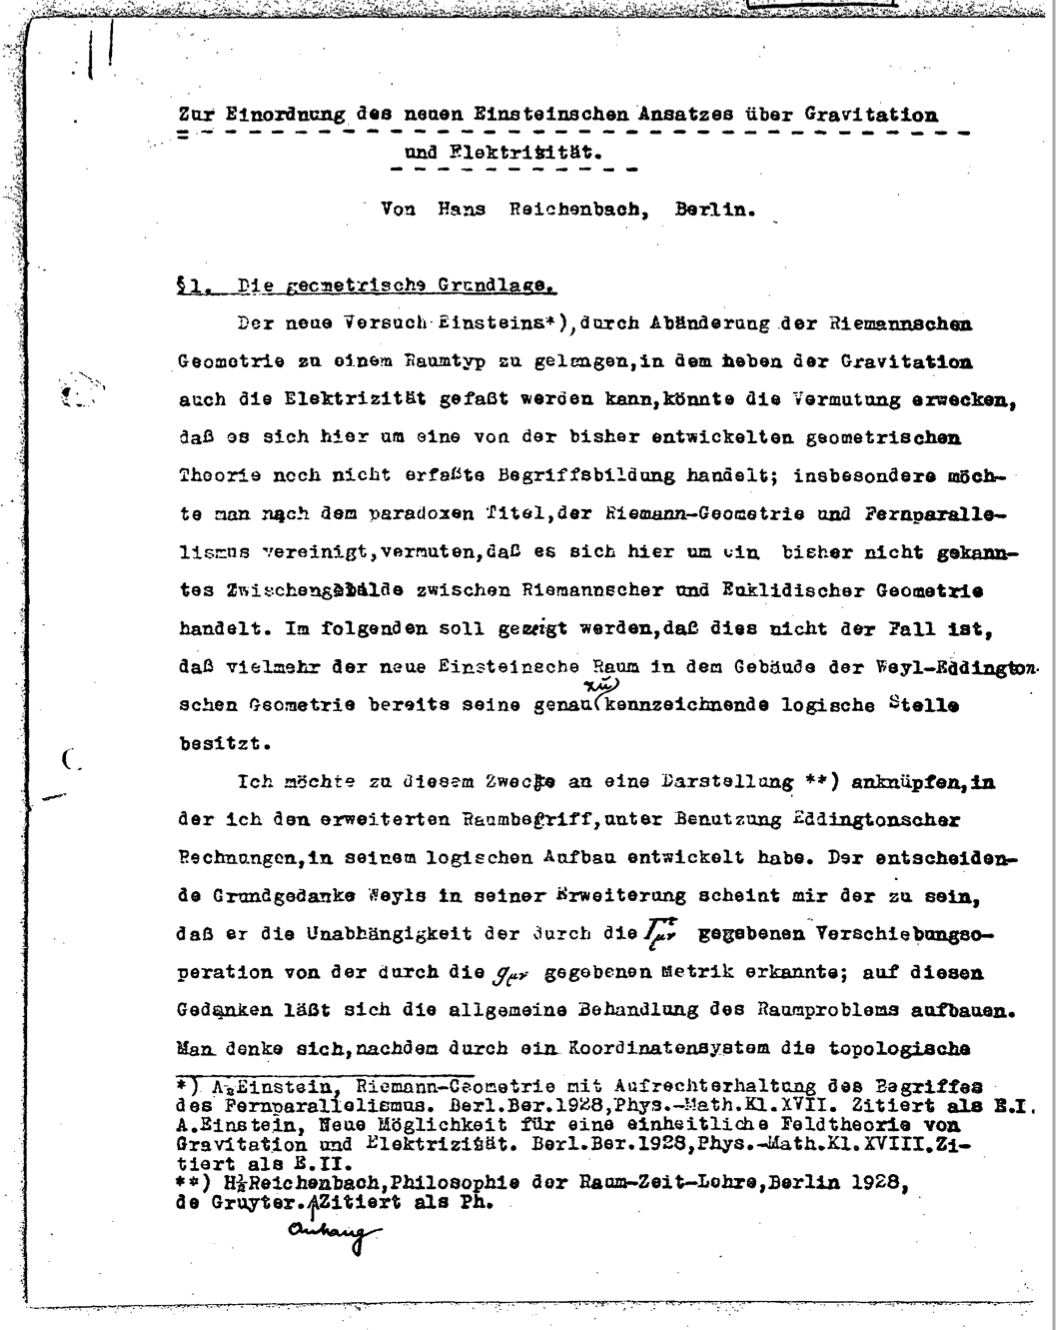
\includegraphics[scale=0.25]{1928ReichebachTele.png}
\caption{\label{fig:reichenbachfirst} First page of Reichenbach's manuscript \citep{Reichenbach1928b}}
\end{figure}

According to Reichenbach, a \q{real physical achievement is obtained only if, moreover, the operation of displacement is filled with physical content} \manu{7}. Einstein's geometry, being flat, implies the existence of a straight line, a line of which all elements are parallel to each other, which is nevertheless not identical with a geodesic \citep[224]{Einstein19282}. However, as Reichenbach reported, the latter has no physical meaning in Einstein's theory. As a \scare{geometrical interpretation}, Reichenbach concluded, then his \S49-theory was preferable since the straightest lines and shortest line correspond to the motion of charged and uncharged test particles under the influence of the combined gravitational-electromagnetic field. Once again, Einstein's goal was to use this geometrical apparatus as a starting point to find the right \scare{action}, from which a set of field equations could be derived. However, Reichenbach commented, nothing new came out of it: \q{[T]he derivation of the Maxwellian and gravitational equation from a variational principle was already achieved by other approaches} \manu{6}, like, say, Einstein--Eddington purely affine theory. 



In the subsequent letter, Einstein defended his classification of geometries but did not comment on Reichenbach's objection. However, he invited Reichenbach and his first wife, Elisabeth, for a cup of tea on \datef{5}{11}{1928}. During this meeting, Einstein might have informed Reichenbach about abandoning the variational strategy to find the field equations \citep{Sauer2006}. It is also probable that Einstein explained to Reichenbach that his goal was \emph{not} to provide a \emph{geometrization} of the electromagnetic field, but to provide their \emph{unification} of both fields. Therefore, Einstein's choice of field structure was not motivated by geometrical considerations, nor did it have a geometrical meaning. The goal was to recover a set of field equations that yielded the classical equations of gravitation and electromagnetism only to the first order. In other words, the theory should predict \emph{new} effects in the case of strong fields. To obtain this result, Einstein was ready to adopt a whatever-it-takes strategy. He was not only willing to forgo any physical interpretation of the fundamental variables of the theory, but he was also ready to abandon the variational approach as he was doing in the paper he was working on. 

It is hard to imagine that the divergence of their philosophical views did not emerge during those discussions. In a semi-popular paper Einstein had submitted a few weeks later \citep[131]{Einstein1929}. Einstein insisted on the speculative nature of the new theory. One starts from this mathematical structure and then searches for the simplest and most natural field equations that the \vbein-field can satisfy \citep[131]{Einstein1929}. The physical soundness of the field equations can be confirmed only by integrating them, finding particle solutions, and the laws governing their motions in the field. However, this was a challenging task. Einstein warned his readers of the dangers of proceeding \q{along this speculative road} \citep[127]{Einstein1929}. \qt{Meyerson's comparison with Hegel's program \origins{Zielsetzung}}, Einstein put it in a footnote, \qt{illuminates clearly the danger that one here has to fear}{Meyersons Vergleich mit Hegels Zielsetzung hat sicher eine gewisse Berechtigung; er beleuchtet hell, die hier zu fürchtende Gefahr} \citep[127]{Einstein1929}.

\subsection{Reichenbach's Articles on \FP field theory}
%
In the late 1920s, Reichenbach was a regular contributor to the \jt{Vossische Zeitung}, at that time Germany's most prestigious newspaper; not surprisingly, he was asked for a comment on Einstein's theory, which had started attracting irrational attention in the daily press \citep[see][346]{Pais1982}. With the advantage of having personally discussed the topic with Einstein a few weeks earlier, Reichenbach published a brief didactic paper on Einstein's theory on \datef{25}{1}{1929} \citep{Reichenbach1929c}. Reichenbach profited from the conversation with Einstein. In particular, it is revealing that Reichenbach did not present Einstein \FP---as it would be more natural in popular writing---as an attempt to \emph{geometrize} the electromagnetic field on par with the previous geometrization gravitational field achieved by \gr. On the contrary, he decided to present \FP as an attempt to \emph{unify} the two separate fields on par with similar unifications operated by special and \gr.

Although the article was fairly innocuous, Einstein was distraught by Reichenbach's decision to leak a private conversation to the press \letteraeap{Einstein}{Vossische Zeitung}{25}{1}{1929}[73-229]. The exchange of the letters that ensued (\lettercpae{Reichenbach}{Einstein}{27}{1}{1929}[16][384], \lettercpae{Einstein}{Reichenbach}{30}{1}{1929}[16][390], \lettercpae{Reichenbach}{Einstein}{31}{1}{1929}[16][391]) put a serious strain in their personal relationships. The disagreement over a seemingly trivial issue appeared to have been accompanied by a feeling of greater intellectual estrangement. Reichenbach's personal correspondence expressed his disappointment with Einstein's breach of their friendship, while his published works reflected his disappointment with Einstein's deviation from their shared philosophical principles. By the time of the article's publication for the \VZ, Reichenbach had already written two papers on the \FP that are both dated \datef{22}{1}{1929} that were published in the following months \citep{Reichenbach1929b,Reichenbach1929a}. These articles are Reichenbach's last contribution to issues related to \rt and \spti theories. On the one hand, Reichenbach applied to Einstein's new theory his ideas about the \uftp as the were presented in the \Ap to the \PRZL  \citep[\S46]{Reichenbach1928}. On the other hand, he introduced novel insights by explicitly distinguishing between the \scare{geometrization program} and the \scare{unification program}

In the first paper for the \citejournal{Reichenbach1929b}, Reichenbach introduced the history of the \uft in an entirely different manner than he had done before. In the \Ap to the \PRZL, the history of the \uft program was ultimately presented as a linear evolution of the geometrization program that had progressively become more abstract. Now Reichenbach---probably following the discussion he had with Einstein in November---describes the history of the \uft as the progressive \emph{decline} of the geometrization program and the concurrent \emph{ascent} of the unification one. After the failure of Weyl's first attempts, most physicists, including Einstein \citeyearp{Einstein1923d,Einstein1925a}, considered it preferable to sacrifice the geometrical interpretation---i.e., to relinquish the coordination of geometrical notion of parallel transport of vectors with the behavior \rac---and then to use the geometrical variables (\Gtmn, $\varphi_\nu$ and so on) as \scare{calculation device} for the greater good of finding the field equations. Reichenbach had come to understand that, in Einstein's view, the aim of the \uftp was not the geometrization of the electromagnetic field alongside the gravitational field; it was the unification of the electromagnetic and gravitational fields. 

%In the second part, Reichenbach introduced the distinction between  \begin{inparaenum}[(a)] \item\label{fu} a formal unification and \item\label{iu} an inductive unification \end{inparaenum}. This distinction seems to be an application of  Reichenbach's more famous classification of two types of simplicity \citepp[9]{Reichenbach1924}[\S11]{Reichenbach1929} to the case of unified field theories. In this way, Reichenbach could describe two opposite approaches to the \uftp. 

Thus, Reichenbach's concern became to explain what \scare{unification} means in this context. The problem was addressed in detail in the more technical paper, which grew out of the manuscript that Reichenbach had sent to Einstein \citep{Reichenbach1929a}.  In this setting, his \S49-theory came in handy. Reichenbach's theory uses a similar geometrical setting as Einstein's theory. Both use a non-symmetric affine connection. In Einstein's approach, the further conditions that the geometry is flat are imposed, allowing for distant parallelism. According to Reichenbach, his \S49-theory was able to provide a \emph{proper} geometrical interpretation of the combined gravitational/electromagnetic field. However, the theory could achieve only a \emph{formal unification} because no new testable predictions were made:

\qt{The author \textins{Reichenbach} has shown that the first way can be realized in the sense of a combination of gravitation and electricity to one field, which determines the geometry of an extended Riemannian space; it is remarkable that thereby \myemph{the operation of displacement receives an immediate geometrical interpretation, via the law of motion of electrically charged mass-points}. The straightest line is identified with the path of electrically charged mass points, whereas the shortest line remains those of uncharged mass points. In this way, one achieves \myemph{a certain parallelism to Einstein's equivalence principle}. By the way, [the theory introduces] a space 
cognate to the one used by Einstein, i.e., a metric space with non-symmetrical \Gtmn. The aim was to show that the geometrical interpretation of electricity does not mean a physical value of knowledge per se}{Daß der erste Weg durchführbar ist im Sinne einer Zusammenfassung yon Gravitation und Elektrizität zu einem Feld, welches die Geometrie in einem erweiterten Riemannschen Raum bestimmt, ist vom Verfasser gezeigt worden; es ist bemerkenswert, daß dabei die Verschiebungsoperation eine unmittelbare geometrische Deutung finden kann, nämlich durch das Bewegungsgesetz elektrisch geladener Massenpunkte. Es wird dort die geradeste Linie mit der Bahn des elektrisch geladenen Massenpunkts identifiziert, während die kürzeste Linie die des ungeladenen Massenpunkts bleibt. Hierdurch wird eine gewisse ParallelRat zu dem Einsteinschen-Aquivalenzprinzip erreicht. ?brigens wird dort ein dem Einstein'schen Raum verwandter Raum, nämlich ein metrischer Raum mit unsymmetrischen \Gtmn zugrunde gelegt. Absicht nämlich, zu zeigen, daß geometrische Deutung der Elektrizität an sich noch keinen physikalischen Erkenntniswert bedeutet}[688\me][Reichenbach1929a]
%
Suppose one wants to give a geometrical interpretation of a combined gravitational/electromagnetic field using the affine connection \Gtmn as a fundamental variable. In that case, one should provide a coordinate definition of the operation of parallel displacement of vectors before starting to search for the field equations. Otherwise, it is hard to understand how one could test whether the latter made correct predictions. Reichenbach's theory was meant to show that a successful geometrical interpretation of this kind can always be achieved with some mathematical trickery. However, more than a successful geometrization is required to achieve a substantive unification. For Reichenbach, this should have been a warning that the very hope that the geometrical interpretation of a physical field was the key to new physical insights was misplaced. 

Einstein \FP-field theory is an instance of a second approach, which claims to achieve an \emph{inductive unification}, by forgoing the geometrical interpretation, that is, without providing a physical meaning of the \Gtmn in terms of the motion of test particles:

\qt{On the contrary, Einstein's approach of course uses the second way, since it is a matter of increasing physical knowledge; it is the goal of Einstein's new theory to find such a concatenation of gravitation and electricity, that only in first approximation it is split in the different equations of the present theory, while is in higher approximation reveals a reciprocal influence of both fields, which could possibly lead to the understanding of unsolved questions, like the quantum puzzle. However, it seems that this goal can be achieved only \myemph{if one dispenses with an immediate interpretation of the displacement, and even of the field quantities themselves}. From a geometrical point of view this approach looks very unsatisfying. Its justification lies only on the fact that the above mentioned concatenation implies more physical facts that those that were needed to establish it }{Der Einsteinsche Ansatz benutzt dagegen natürlich den zweiten Weg, denn ihm ist es ja um Vermehrung des physikalischen Wissens zu tun; es ist als Ziel der neuen Theorie Einsteins, eine derartige Verkettung yon Gravitation und Elektrizität zu finden, daß sie nur in erster Näherung in die getrennten Gleichungen der bisherigen Theorie zerspaltet, während sie in höherer Näherung einen gegenseitigen Einfluss beider Felder lehrt, der möglicherweise zum Verständnis bisher ungelöster Fragen, wie der Quantenrätsel, führt. Aber dieses Ziel scheint nur erreichbar zu sein unter Verzieht auf eine unmittelbare physikalische Interpretation der Verschiebungsoperation, ja sogar der eigentlichen Feldgrössen selbst. Vom geometrischen Standpunkt als deshalb ein solcher Weg sehr unbefriedigend erscheinen; seine Rechtfertigung wird allein dadurch gegeben werden können, daß er durch die genannte Verkettung mehr physikalische Tatsachen umschließt, als zu seiner Aufstellung in ihn hineingelegt wurden}[688\me][Reichenbach1929a]
%
In Reichenbach's view, \FP appeared not only as a formally satisfying unification but also as a genuine advance over the available theories. It entails some coupling between the electromagnetic and gravitational fields that was not present in the given individual field theories. However, Reichenbach argues that Einstein could only achieve this result at the expense of a physical interpretation of the fundamental geometrical variables. As we have seen, Einstein's flat affine connection \Gtmn defines a set of straight lines as privileged paths; however, these lines are not interpreted as paths of particles \citep[23]{Einstein1930i}. Before integrating the field equations, the laws governing the latter are unknown (\letter{Einstein}{Cartan}{7}{1}{1930}[A-XVI][Debever1979]). Consequently, the theory cannot be confirmed or disproved experimentally by observing the behavior of suitable indicators.

In Reichenbach's diagnoses, the stagnation of the \uftp depended on the presence of a sort of trade-off between geometrization and unification of which physicists were only partially aware. \Gr was the only theory that was able to combine both virtues: \begin{inparaenum}[(1)] \item the theory provided a proper \emph{geometrical interpretation} of the gravitational field because it introduced a coordinative definition of the field variables \gmn, in terms of the behavior of those that were traditionally considered geometrical measuring instruments, such as \rac, light rays, free-falling particles \item the theory provided a \emph{proper unification} by predicting that the gravitational field had specific effects on such measuring instruments that were not implied by previous theories of gravitation---such as gravitational time dilation \end{inparaenum} \citep[378]{Reichenbach1928}. Successive attempts to include the electromagnetic field in the framework of general relativistic field theory failed to uphold this standard. 

%According to Reichenbach

According to Reichenbach, the reason for this failure was ultimately not hard to pinpoint. The effective interplay between geometrization and unification did not seem reproducible without a proper analogon of \emph{equivalence principle}. Without the equivalence principle, a further geometrization of electromagnetic fields was not worth pursuing since it had no physical justification\footnote{see \cref{pauli}}. Einstein could counter these objections by claiming that geometrization had never been the goal. The achievement \gr was to have combined inertial and gravitational just like \sr has combined magnetic and electric field as components of a unified field structure. However, without an analogon of the equivalence principle, there seems to be also no physical justification for searching for further unification of the electromagnetic and gravitational field. Nevertheless, Einstein considered the separation between the two fields as theoretically unbearable \citep[24]{Einstein1930i}. However, he did not have any physical clue as to what the more comprehensive mathematical structure may be, in which the electromagnetic and gravitational fields will appear as two sides of the same field. Hence, Einstein had no choice but to turn to the criterion of mathematical simplicity, which was challenging to define with precision.

To Reichenbach's dismay, Einstein had abandoned the \emph{physical heuristic}\footnote{For Einstein's earlier \s{logic of discovery}, see \cite{Giovanelli2020a}} that leads him to \gr in the name of a \emph{mathematical heuristic} that was not different from Weyl's speculative approach that he had dismissed a decade earlier. As we have seen, as early as in his habilitation, he considered the great achievement of \rt the \emph{separation of mathematical necessity and physical reality}. Reichenbach had always perceived this separation as nothing more than a philosophical distillation of Einstein's scientific practice. However, in the search for a \uft, Einstein had come implicitly to question this distinction, coming close to a plea for a \emph{reduction of physical reality to mathematical necessity}. Einstein put it candidly in his Stodola-\german{Festschrift}'s contribution---that he sent for publication toward the end of January \lettercpaeabsp{Einstein}{Honegger}{30}{1}{1929}[864]. The ultimate goal of understanding reality is achieved when one could prove that \qt{even God \myemph{could not have established these connections otherwise} than they actually are, just as little as it would have been in his power to make the number 4 a prime number}{selbst Gott jene Zusammenhänge nicht anders hätte festlegen können, als sie tatsächHch sind, ebensowenig, als es in seiner Macht gelegen wäre, die Zahl 4 zu einer Primzahl zu machen} \citep[127]{Einstein1929}.

\section{Conclusion}
%
After the publication of the new derivation of the \FP-field equations in January 1929 \citep{Einstein1929b}, Einstein wrote a popular account of the theory for the \jt{New York Times} and \jt{The Times} of London \citepp{Einstein1929-2-3}{Einstein1929-2-4}[also published as][]{Einstein1930h}. In this article, Einstein emphasized the highly speculative nature of \uftp, without hesitating to endorse Meyerson's somewhat outrageous comparison with Hegel. It is difficult to deny the symbolic significance of Einstein's decision to mention Meyerson rather than Reichenbach as a philosophical interlocutor in an article with such a vast readership. After a decade of personal friendship and intellectual collaboration, Einstein appears to have questioned the very core of his early philosophical alliance with Reichenbach. While Reichenbach considered the separation between mathematics and physics the great achievement of the \rt, Einstein regarded mathematics itself as the key to accessing the structure of the \scare{total field}.

Although Einstein's \FP attracted the attention of mathematicians, Reichenbach's skepticism was shared by the physics community\footnote{Weyl, whom Einstein had always scolded for his speculative style of doing physics, could relaunch the accusation in a paper \citep{Weyl1929c} in which he had uncovered the gauge symmetry of the Dirac theory of the electron \citepp{Dirac1928}{Dirac1928b}. \q{The hour of your revenge has come}, Pauli wrote to Weyl in August: \qt{Einstein has dropped the ball of distant parallelism, which is also pure mathematics and has nothing to do with physics and \emph{you} can scold him}{jetzt hat Einstein den Bock des Fernparallelismus geschossenf , der auch nur reine Mathematik ist und nichts mit Physik zu tun hat, und Sie konnen schimpfen} \letterpaulip{Pauli}{Weyl}{26}{8}{1929}[235]. As Pauli complained, writing to Einstein's close friend Paul \Ehr, \q{God seems to have left Einstein entirely!} \letterpaulip{Pauli}{\Ehr}{29}{9}{1929}[237]}. Einstein was well aware of the marginality of his position, but throughout 1929, he continued to express his confidence in the \FP-program. He defended the theory in public talks \citep{Einstein1930,Einstein1930a,Einstein1930b} as well as in private correspondence (\letterpauli{Pauli}{Einstein}{19}{12}{1929}[239]; \letterpauli{Einstein}{Pauli}{19}{12}{1929}[140]). However, only a few months later, Einstein and Walther Mayer presented a new approach \citep{Einstein1931}, which generalized the \nbein formalism to five dimensions. The optimism faded quickly again, as the theory was unable to solve the matter problem. In a popular talk given in Vienna around mid-October 1931, Einstein resigned himself to describing his field-theoretical work since \gr as a \qt{cemetery of buried hopes}{Friedhof von Begrabener Hoffnungen} \citep[441]{Einstein1932b}\footnote{It is interesting to notice that one of the reasons that induced Einstein to abandon the theory was not dissimilar to Reichenbach's criticism: \q{The main reason for the uselessness of the distant parallelism construction lies, I feel, in that one can attribute absolutely no physical meaning to the \scare{straight lines} of the theory, while the physically meaningful (macroscopic) equations of motion cannot be obtained from it ${ }^{3}$. In other words, the $h_{s v}$ give rise to no useful representation of the electromagnetic field} \letterp{Einstein}{Cartan}{21}{5}{1932}[A XXXV][Debever1979]. Thus, for Einstein, it was legitimate to abandon the physical interpretation of straight lines from the outset if the theory provided a way to derive the laws of motion of the electrons}.

However, Einstein's philosophical motivation for continuing on this path has not changed. Many of his former philosophical allies considered this attitude hard to fathom \citep[215f.]{Frank1947}. However, Einstein's 1933 Oxford lecture address leaves no room for doubt. Einstein's quest for unification, he insisted, was motivated by the deep-seated conviction that \q{nature is the realization of the most simple mathematical ideas} \citep{Einstein1933}. Einstein conceded that experience remains the sole criterion of the physical adequateness of a mathematical construction. However, he insisted that the true creative role belongs to mathematics: \q{I hold it to be true that pure thought is competent to comprehend the real, as the ancients dreamed} \citep[167]{Einstein1933}. After all, he now claims, the search for field theories has always followed the same heuristic pattern: \q{the theorist's hope of grasping the real in all its depth} lies \q{in the limited number of the mathematically existent simple field types, and the simple equations possible between them} \citep[168]{Einstein1933}. Maxwell's equations are the simplest laws for an antisymmetric tensor field derived from a vector; Einstein's equations are the simplest equations for the metric tensor\etc. This strategy applies to Einstein's last attempt at a \uft on a theory based on semi-vectors \citep{Einstein1932c,Einstein1933c,Einstein1934b,Einstein1933d}. After ordinary vectors, the latter are the simplest mathematical fields that are possible in four dimensions and seem to describe certain elementary particles' properties \citep{Dongen2004}. One has to search for the simplest laws these semi-vectors satisfy \citep[168]{Einstein1933}.

In September 1933, three months after the Oxford lecture, Einstein left Europe for Princeton. Reichenbach started to teach at the University of Istanbul in the Fall of the same year. He tried to obtain a position at Princeton a few years later \citep{Verhaegh2020a}. However, Reichenbach was concerned about Weyl's possible opposition: \q{He is my adversary since a long time,} he wrote to Charles W.\ Morris: a supporter of a form a \q{mathematical mysticism} that was \q{very much opposed to my empiricist interpretation of relativity} \letterhrp{Reichenbach}{Morris}{12}{4}{1936}[013-50-78]. Thus, in April 1936, Reichenbach turned to Einstein to ask for his support. \q{More than 10 years ago}, he explained, \qt{Herr Weyl spoke out very negatively about my work on the theory of relativity}{Herr Weyl hat sich vor mehr als 1o Jahren sehr ablehnend iiber meine Arbeiten zur Relativitat6theorie ausgesprochen}. Reichenbach feared that \qt{Weyl's opposition persists to these days}{Ich vermute, daB Herrn Weyls Gegnerschaft noch heute fortdauert, und darum ware ich Ihnen sehr dankbar, wenn Sie da zu meinen Günsten eintreten kGnnten} \letteraeap{Reichenbach}{Einstein}{12}{4}{1936}[20-107]. Reichenbach might have had good reasons for turning to Einstein's help against Weyl in academic matters. However, it is worth noticing that, by that time, Reichenbach might have been closer to Weyl than to Einstein in scientific matters. A decade later, the roles were reversed. In the late 1930s, Weyl, like Reichenbach, had utterly lost confidence in the \q{geometrical leap \origins{Luftsprünge}} of the early 1920s\footnote{In a way not dissimilar to Reichenbach, Weyl considered early unified field theories as \q{merely geometrical dressings (\german{geometrische Einkleidungen}) rather than as proper geometrical theories of electricity}.
\citep[343]{Weyl1931}}, and felt the need to \q{return to the solid ground of physical facts} \citep[343]{Weyl1931}, to the vast amount of experimental data provided by spectroscopy. On the contrary, gravitational research had turned Einstein into a \scare{believing rationalist} \citep{Ryckman2014}, convinced that physical truth lies in mathematical simplicity \letteraeap{Einstein}{Lanczos}{24}{1}{1938}[15-268].

%%turned from his speculative and strongly idealist approach of the 1920s, to a mathematically empiristic and moderately materialistic by the 1930s .
%
%
%
%
%
%
%
%Einstein replied disillusioned that he had heard from Rudolf Carnap that even Princeton did not want to hire more Jewish intellectuals (\letter{Einstein}{Reichenbach}{2}{5}{1936}[20-118][EA]).

In 1938, Reichenbach finally managed to move to the United States \citep{Verhaegh2020a}. Soon after, he and Einstein resumed their epistolary contact to support Bertrand Russell, who had been dismissed from the City College of New York due to his anti-religious stance (\letteraea{Reichenbach}{Einstein}{14}{8}{1940}[20-127]; \letteraea{Einstein}{Reichenbach}{22}{8}{1940}[20-110]). Later, both Reichenbach and Einstein contributed to a volume honoring Russell for the series \textit{Library of Living Philosophers}, edited by Paul \citet{Schilpp1944}. Reichenbach was also asked to contribute to a similar volume in honor of Einstein a few years later \citep{Schilpp1949}.  In some unpublished notes about \citets{Reichenbach1949} contribution, \citet{Einstein1949f} praised him his rare ability for combing breath of knowledge with clarity \hide{the universality of knowledge by sacrificing clarity} \hide{Hans Richenbach von so viclen sei.ner hollogen auszeichnet, 1st der Umstand, dass er Allgomeinheit der Erenntnis niemals erkauft durch Opferung der Klerheit. br sieht in der logischen Kritik der Lehren und liethoden der FinzelWissenschaften die Hauptaufgabe der Philosophie} \citep{Einstein1949f}. However, Einstein ultimately disagreed with many of Reichenbach's philosophical tenets. In particular, Reichenbach's claim that \qt{\scare{\emph{the meaning of a statement is reducible to its verifiability}}\footnote{In English in the text}}{Dann erschetnt ueberhaupt die These problematisch "the meaning of a statement is reducible to its verifiabilitys} appeared to Einstein problematic; he found \qt{dubious whether this conception of \scare{\emph{meaning}}\footnote{In English in the text} can be applied to the single \emph{statement}\footnote{In English in the text}}{ss erscheint naemlich zweifelhaft, ob man an dieser Auffassung von "meaning" fuer das einzelne statement festhalten karn} \citep{Einstein1949f}. 

As is well known, in the so-called \scare{Reply to criticisms} \citep{Einstein1949a} included in the Schilpp-volume, Einstein reformulated this line of argument by staging a dialogue between Reichenbach-Helmholtz, Poincaré, and an anonymous non-positivists, who claims that geometry and physics can be compared with experience only as a whole \citep[676f.]{Einstein1949a}. The question at stake, as Einstein put it jokingly, was nothing but Pilates's famous question \scare{What is truth?} \parencite[John 18:38, quoted in][676]{Einstein1949a}. Although this dialogue has become enormously famous, its meaning has been ultimately misunderstood. Einstein was not engaging in a philosophical digression about the 19th-century debate on the foundation of geometry. The question what it means for a theory to be \scare{true} was ultimately motivated by his tireless pursuit of the theory of the \scare{total field}. 

At that time, Einstein had returned to his 1925 metric-affine approach introducing non-symmetric \gmn and \Gtmn as fundamental variables \citep{Einstein1945,Einstein1945-04}. In private correspondence, Einstein's long-life friend Michele Besso raised against Einstein objections similar to those that Reichenbach had advanced over twenty years earlier against the same theory. The symmetric part of the \gmn and the corresponding \Gtmn, Besso claimed, should define the straightest line, which is also the shortest. Do these lines represent the trajectories of test particles? What is their physical meaning? \letterspezialip{Besso}{Einstein}{11}{4}{1950}[171]. Einstein's reply reveals his fundamental philosophical conundrum:

\qt{Your questions are entirely legitimate, but it is not answerable for the time being \textelp{}. This is because there is no real definition of the field in a consistent field theory. This puts you in a Don Quixotic situation, in that you have absolutely no guarantee whether it is ever possible to know if the theory is \scare{true}. \textit{A priori} there is no bridge to empiricism. For example, there isn't a \scare{particle} in the strict sense of the word because the existence of particles doesn't fit the program of representing reality by everywhere continuous \textelp{}. For example, the theory introduces a symmetric \gmn \textelp{} and then a geodesic line. However, from the outset, one has no clue that these lines have any physical meaning, not even approximately \textelp{} It boils down to the fact that a comparison with what is empirically known can only be expected from the fact that strict solutions of the system of equations can be expected found, that reproduce the behavior of empirically \scare{known} structures and their interactions. Since this is extremely difficult, contemporary physicists' skeptical attitude is probably entirely understandable. In order to really grasp this conviction of mine, you must read my answer in the anthology \origins{Sammelband}\footnote{\cite{Einstein1949a}} \emph{again and again}}{Deine in dem Brief vom 11.IV gestellten Fragen sind durchaus natürlich, aber his auf Weiteres nicht beantwortbar. Dies liegt daran. dass es in enner Dies liegt daran, dass es in einer konsequenten Theorie des Feldes keine Realdefinition für das Feld gibt. Es ist wahr, dass man dadurch in eine Don Ouixotische Situation kommt, indem man durchaus keine Gewähr dafür hat. dass esjemals möglich ist zu wissen, ob die Theorie ,,wahr“ ist. Es ist a priori keine Brücke zur Empirie gegeben. Es gibt z.B. nicht ein „Teilchen im strengen Sinne des Wortes, weil dies nicht zu dem Programm passt; die Realität durch überall kontinuierliche, ja sogar analytische Funktione 4zu repräsentieren. In der Theorie gibt es z.B. ein symmetrisches \gmn geodätische Linie. Aber man hat von vorneherein gar keinen Anhaltspunk dafür, dass diesen Linien irgend eine physikalische Bedeutung zukommt, auch nicht approximativ \textelp{} Es kommt darauf hinaus, dass ein Vergleich mit empirisch Bekanntem nur davon erwartet werden kann, dass man strenge Lösungen des Glei­ chungssystems findet, in denen sich empirisch „bekannte“ Gebilde und ihre Wechselwirkungen „ spielgeln D a dies ungeheuer schwer ist, ist die skep­ tische Haltung der zeitgenössischen Physiker wohl zu verstehen nicht näher kommt. Um diese meine Ueberzeugung wirklich zu begreifen, musst Du meine Antwort in dem Sammelband}[\letterspezialip{Einstein}{Besso}{15}{4}{1950}[172]]
%
This passage summarizes many of the issues that Reichenbach and Einstein had discussed over the years. It explains Reichenbach's legitimate concern that geometrical concepts of the theory, like that of the straightest lines, should receive a physical interpretation from the outset in terms of the motion of test particles. However, it also explains why Einstein did not find this approach viable in pursuing a theory in which there are \latin{stricto sensu} no particles. Usually, a field is defined in the first place by the forces that it exerts on test particles. However, discovering this force law requires the integration of the field equations. It is in this context that question of the \scare{truth} of a theory of this kind could not be avoided. It was ultimately this question that Reichenbach and Einstein had discussed for over 30 years. Whereas Einstein was ready to change his conception of \scare{truth} for the search of the \uft, Reichenbach urged Einstein to abandon this search in the name of a once shared conception of the \scare{truth} of a physical theory.

% In this context there is no separation between empty scheme, and the coordinative defintions. The of mathematical si, was not only a non-positivist, he was a tamed metaphysician

%The principle of \scare{logical simplicity} as a criterion for the choice of the right set of equations \citep[120]{Einstein1950e}. \q{What most simple property can be required from what most simple object (field) while pre­ serving the principle of general relativi­ty?} \citep[15]{Einstein1950}. 


\printshorthands
\printbibliography

\end{document}